

\title{\LARGE \bf
Dimensionless Policies based on the Buckingham $\pi$ Theorem: \\ 
Is it a good way to Generalize Numerical Results?
}


%\author{Alexandre~Girard,~\IEEEmembership{Member,~IEEE,}
%        and~H.~Harry~Asada,~\IEEEmembership{Member,~IEEE}% <-this % stops a space
\author{Alexandre Girard$^{1}$% <-this % stops a space
\thanks{$^{1}$Alexandre Girard is with the Department of Mechanical Engineering, Universite de Sherbrooke, Qc, Canada {\tt\small  alex.girard@usherbrooke.ca }}% <-this % stops a space
}%


% make the title area
\maketitle
\thispagestyle{empty}
\pagestyle{empty}


\begin{abstract}
Yes if the context, the list of variables defining the motion control problem, is dimensionally similar. Here we show that by modifying the problem formulation using dimensionless variables, we can re-use the optimal control law generated numerically for a specific system to a sub-space of dimensionally similar systems. This is demonstrated, with numerically generated optimal controllers, for the classic motion control problem of swinging-up a torque-limited inverted pendulum. %The dimensional analysis also show that multiple systems of various dimensions can share a data-base for reinforcement learning. %TODO: (We also demonstrate that by leveraging this scheme when using reinforcement learning, multiple systems of various dimentions can share a data-base during the learning phase, which can be a big advantage for data efficiency.) 
We also discuss the concept of regime, a region in the space of context variables, that can help relax the condition on dimensional similarity. 
It remains to be seen if this approach can also help generalizing policies for more complex high-dimensional problems.
\end{abstract}

%%%%%%%%%%%%%%%%%%%%%%%%%%%%%%%%%%%%%%%%%%%%
\section{Introduction}

% \paragraph{Many numerical algorithms = black box mapping}
% -Trajectory optimization
% -Reinforcement learning
% -etc.

% \paragraph{With numerical results, unlike analytical solutions, system and problem parameters are not explicitly in the solution }

% \paragraph{This makes the results "context specific" and makes its harder to generalize }

The state-of-the-art toolbox of control engineers include many numerical algorithms and data-driven schemes. Many control approaches now include a type of mathematical optimization that has no closed-form solution and that is thus solved numerically. More specifically, reinforcement learning (RL), which we can be seen as a data-driven offline optimization, is starting to be a viable option for solving some motion control problems \cite{rudin_learning_2022}. All in all, numerical tool are very useful and have been used to solve many hard control problem. However, they have a major drawback compared to simpler analytical approaches: parameters of the problem are not appearing explicitly in the solutions, which makes it much harder to generalize and reuse them. 

Analytical solutions to control problems have the useful property of allowing the solution to be adjusted to different system parameters by simply substituting the new values in the equation. Most numerical solutions, including RL, usually act has black-boxes with respect to the parameters. For instance, if we use a reinforcement learning (RL) approach to find a good feedback law for a given task with a robot, the solution will be specific to this system. If the RL-generated feedback law is transferred to a robot with a longer arm, there is a good chance it will not behave as intended. With an analytical feedback law solution, we would simply update the value of the length variable in the equation to adjust it, while with a RL solution we would have to re-conduct all the training implying generally multiple hours of data collection and/or computation. It would be a great asset to have the ability to adjust black-box numerical solutions with respect to some problem parameters.  

%%%%%%%%%%%%%%%%%%%%%%
\begin{figure}[t]
% \vspace{-5pt}
\begin{center}
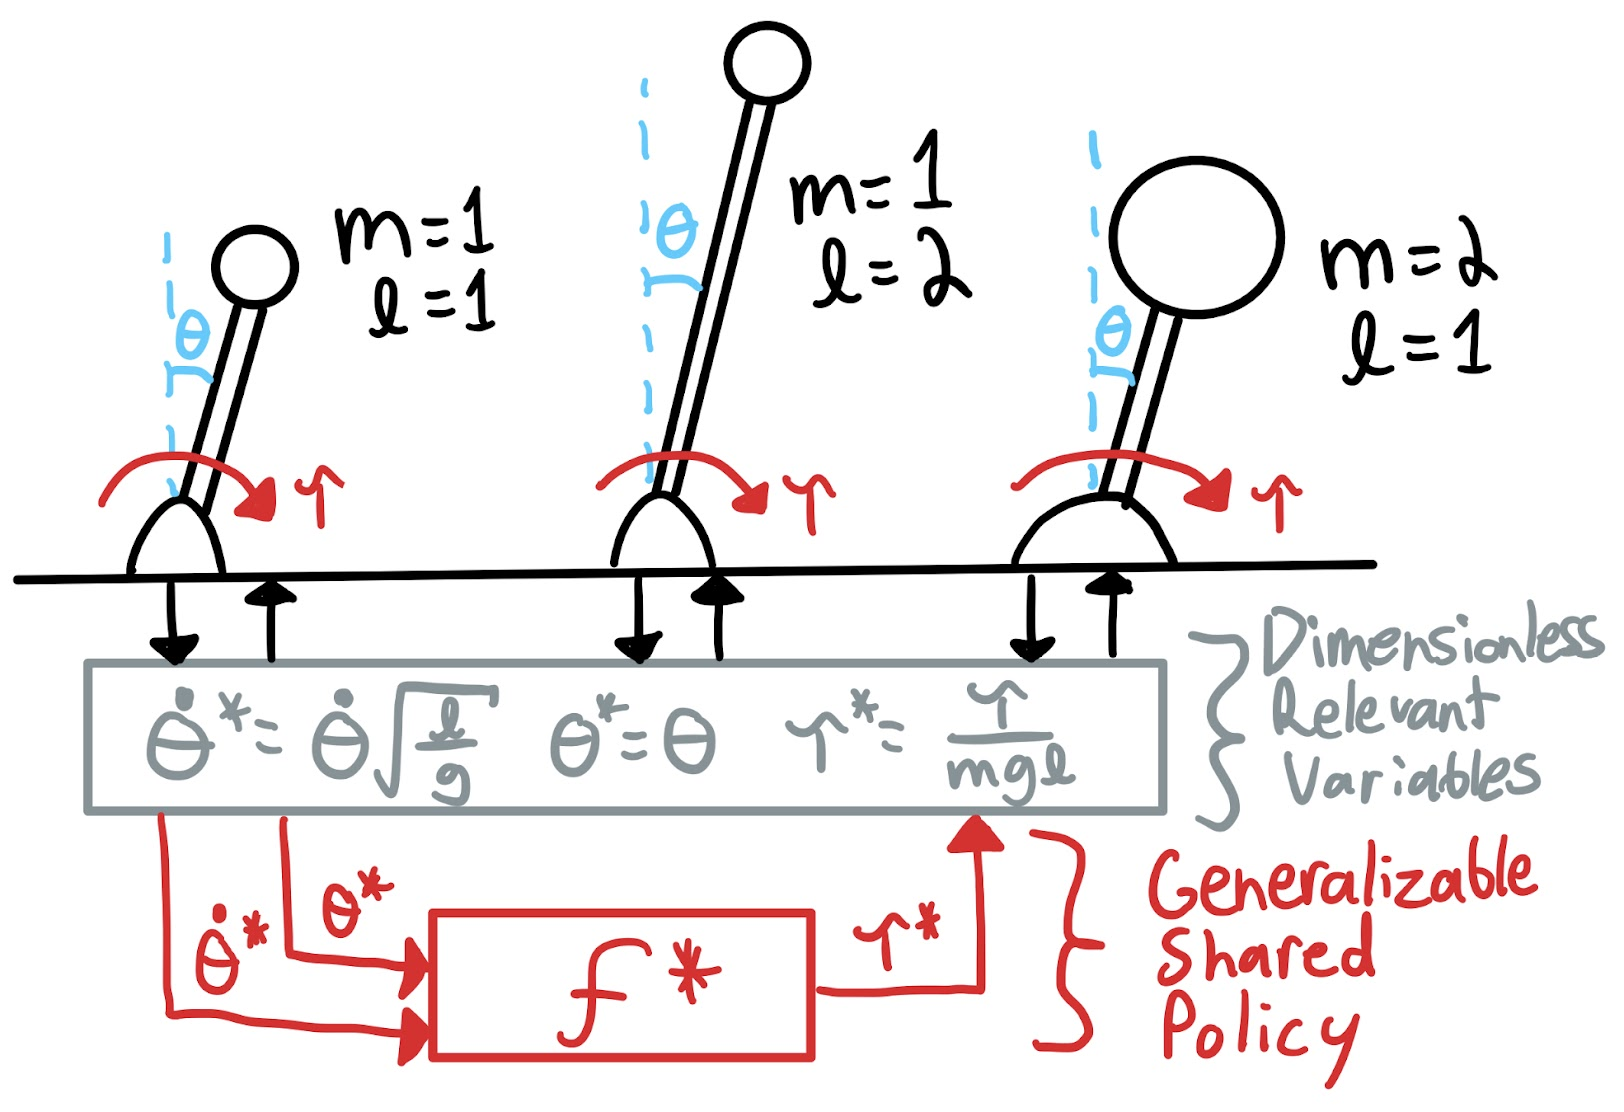
\includegraphics[width=0.99\linewidth]{fig/big_picture3.jpg}
\caption{Shared dimensionless policy for various systems}\label{fig:big_picture}
\end{center}
\vspace{-10pt}
\end{figure}
%%%%%%%%%%%%%%%%%%%%%%

In this paper, we explore the concept of dimensionless policies, a more generic form of knowledge, has a mean to generalize numerical solutions to motion control problems. First, in section \ref{sec:dimenanalysis}, we use dimensional analysis (i.e. the Buckingham $\pi$ theorem) to show that motion control problem with dimensionally similar context variables must share the same feedback law solution when expressed in a dimensionless form, and discuss the implications. Then in section \ref{sec:optimalswingup}, this is demonstrated for the classical motion control problem of swinging-up an inverted pendulum, using numerically generated optimal feedback laws with a dynamic programming algorithm. Also, in section \ref{sec:closedfrom}, we illustrate with two examples that the proposed dimensional scaling is equivalent to changing parameters in an analytical solution. 

%Another aspect to this issue for RL, is the constraint it pose on data during a training phase. 

% \section{Background}

% In the field of learning, this is fall under the vast on-goin challenge of generalizing knowledge...

% more specifically in robot, .. transfer learning..

% ALso, representation learning...

% Usage of Buckingham Pi \cite{bakarji_dimensionally_2022}


% \section{Contribution}








%%%%%%%%%%%%%%%%%%%%%%%%%%%%%%%%%%%%%%%%%%%%
\section{Dimensionless Policies}
\label{sec:dimenanalysis}

In the following section, we develop the concept of dimensionless policies based on the Buckingham $\pi$ and show that multiple motion control problems will have the same policy solution when restated in a dimensionless form, if they have a dimensionally similar context.

%%%%%%%%%%%%%%%%%%%%%%%%%%%%%%%%%%%%%%%%%%%%
\subsection{Context variables in the policy mapping}

Here, we will call a feedback law a mapping noted $f$, specific to a given system, from an vector space representing the state $x$ of the dynamic system, to a vector space representing the control inputs $u$ of the system:
%%%%%%%%%%%%%%%%%%%%%%
\begin{equation}
u
=
f \left(
x
\right)
\end{equation}
%%%%%%%%%%%%%%%%%%%%%%
Under some assumptions, mainly a fully observable systems, an additive cost and an infinite time horizon, the optimal feedback law is guarantee to be in this state feedback form \cite{bertsekas_dynamic_2012}. We will only consider this case in the following analysis.

To consider the question of how can this system-specific feedback law be transferred in a different context, it is useful to think about a higher dimension mapping, that we will call a policy and note $\pi$, also having as additional input arguments, a vector of variables $c$ describing the context:
%%%%%%%%%%%%%%%%%%%%%%
\begin{equation}
u
=
\pi \left(
x,
c
\right)
\end{equation}
%%%%%%%%%%%%%%%%%%%%%%
where the context $c$ is the vector of all variables that would affect what is the feedback law solution. We can think about the policy $\pi$ as the solution to a motion control problem, and $c$ as a vector of parameters in the problem definition. The policy $\pi$ outputs the control action as a function of the state $x$, but also of problem parameters. The policy $\pi$ thus contains the feedback laws for all possible contexts. For example, in section \ref{sec:optimalswingup} a case study is conducted considering the optimal feedback law for swinging-up a torque-limited inverted pendulum. For this example, the context variables are the pendulum mass $m$, the gravitational constant $g$, the length $l$, but also what we will call task parameters: a parameter in the cost function $q$ and a constraint $\tau_{max}$ on the maximum input torque, see Fig. \ref{fig:policy_context}. For a given state of the system, the torque policy might be different if any of the context variable change value, for instance if the pendulum is heavier, more torque limited, etc.
%%%%%%%%%%%%%%%%%%%%%%
\begin{figure}[htb]
\vspace{-5pt}
\begin{center}
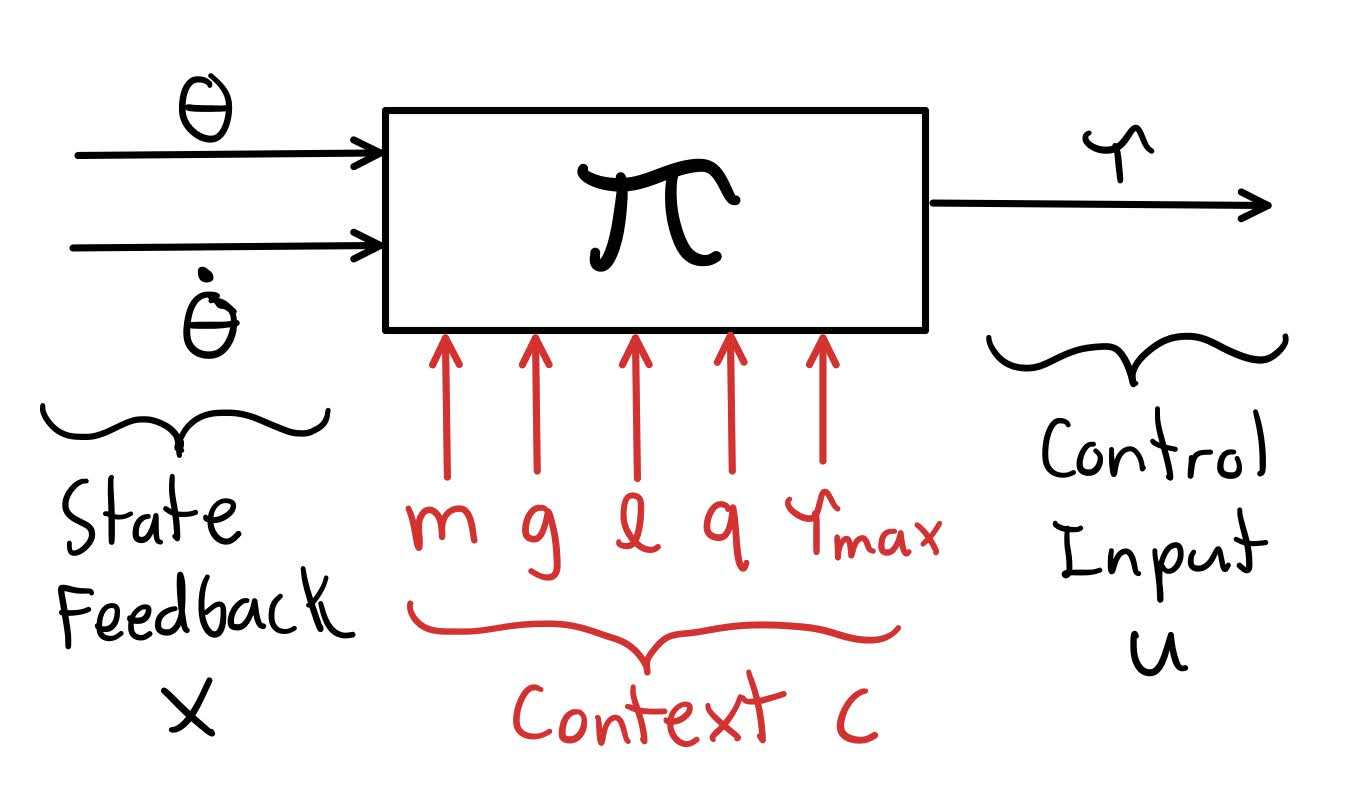
\includegraphics[width=0.75\linewidth]{fig/policy_context2.jpg}
\caption{For the pendulum swing-up control problem, the context includes 5 variables: the parameter of the system: $m$, $g$, and $l$, a parameter of the cost function: $q$ and a parameter defining the constraints: $\tau_{max}$. 
}\label{fig:policy_context}
\end{center}
\vspace{-5pt}
\end{figure}
%%%%%%%%%%%%%%%%%%%%%%
%%%%%%%%%%%%%%%%%%%%%%
\begin{figure}[htb]
\vspace{-5pt}
\begin{center}
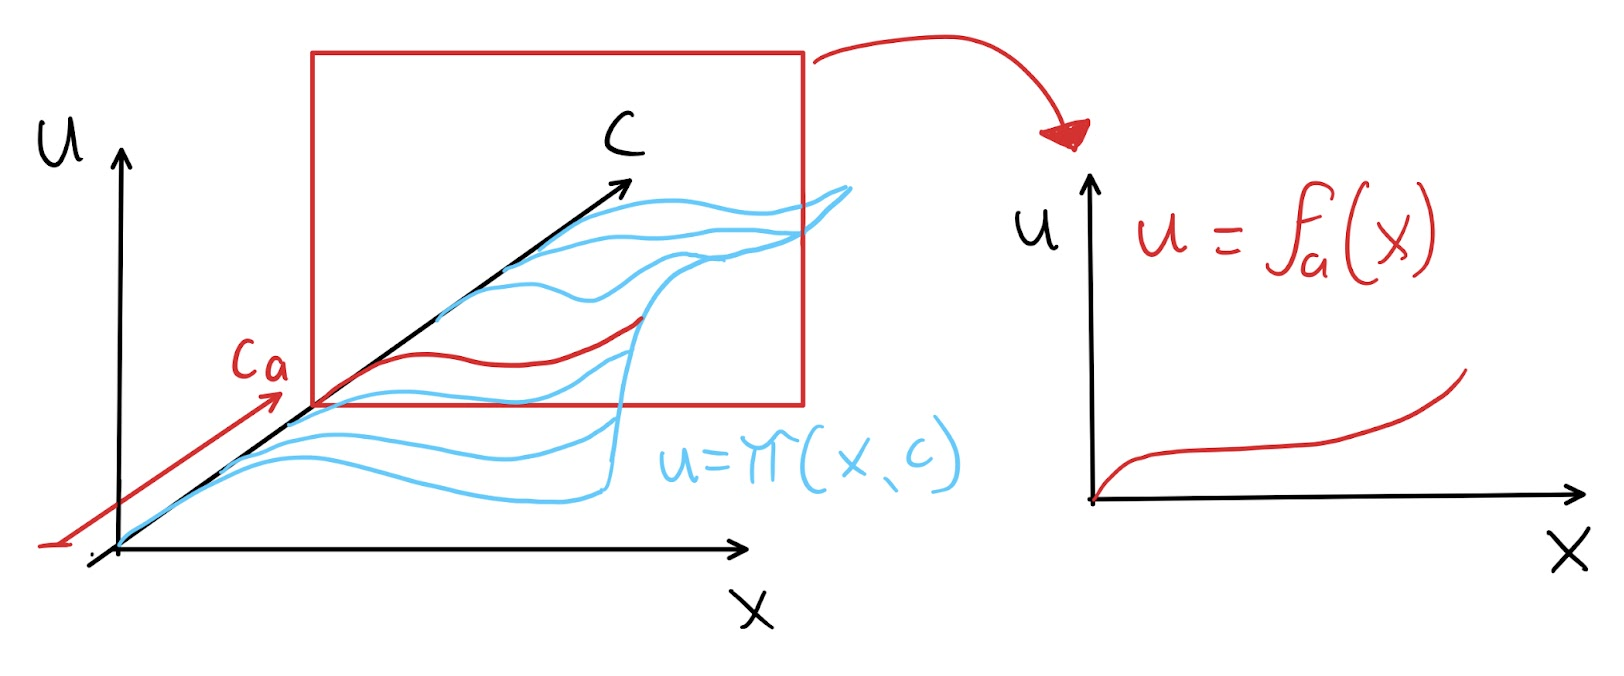
\includegraphics[width=0.95\linewidth]{fig/slice2.jpg}
\caption{A feedback law $f$, is a slice of the higher dimensional policy mapping $\pi$ for a specific context.
}\label{fig:slice}
\end{center}
\vspace{-5pt}
\end{figure}
%%%%%%%%%%%%%%%%%%%%%%

We will use a subscript letter to refer to a specific context, for instance we will note $f_a$ the feedback law solution to a motion problem defined by an instance of context variables $c_a$. The feedback law $f_a$ is thus a slice of the global policy when the context variables are fixed at values $c_a$:
%%%%%%%%%%%%%%%%%%%%%%
\begin{equation}
f_a \left(
x 
\right) 
=
\pi \left(
x,
c = c_a
\right)
\end{equation}
%%%%%%%%%%%%%%%%%%%%%%
as illustrated at Fig. \ref{fig:slice}. Then we can formalize the goal of generalizing a feedback law to a different context: if a feedback law $f_a$ is known for a context $a$ described by variables $c_a$, can this knowledge help finding an equivalent good feedback policy in a different context $c_b$?
%%%%%%%%%%%%%%%%%%%%%%
\begin{equation}
\pi \left(
x,
c = c_a
\right) = 
f_a \left(
x 
\right) 
\quad \Rightarrow \quad
\pi \left(
x,
c = c_b
\right) = ?
\end{equation}
%%%%%%%%%%%%%%%%%%%%%%

Using the Buckingham $\pi$ theorem \cite{buckingham_physically_1914}, we will show that if the context is dimensionnally similar, then both feedback laws must be equal when restated in dimensionless form. It is important to note that for the following dimensional analysis to hold, we must include all the variables, system parameters and task parameters, that would affect the policy solution $\pi$ to the control problem in the context vector $c$:
%%%%%%%%%%%%%%%%%%%%%%
\begin{equation}
\underbrace{\begin{bmatrix}
u_1 \\
\vdots \\
u_k
\end{bmatrix}}_{\text{inputs}}
=
\pi \left(
\underbrace{\begin{bmatrix}
x_1 \\
\vdots \\
x_n
\end{bmatrix}}_{\text{states}}
,
\underbrace{
\underbrace{\begin{bmatrix}
c_1 \\
\vdots \\
\vdots 
\end{bmatrix}}_{\text{system}}
,
\underbrace{\begin{bmatrix}
\vdots \\
c_{m}
\end{bmatrix}}_{\text{task}}
}_{\text{Context $c$}}
\right) 
\label{eq:vectorpolicy}
\end{equation}
%%%%%%%%%%%%%%%%%%%%%%

\subsection{Dimensional analysis of the policy mapping}

For a system with $k$ control inputs, we can treat the augmented policy as $k$ mappings from states and context variables to each scalar control input $u_j$:
%%%%%%%%%%%%%%%%%%%%%%
\begin{equation}
u_j = \pi_j \left(
x_1, \hdots, x_n, 
c_1, \hdots \hdots, c_{m}
\right) 
\label{eq:scalarpolicy}
\end{equation}
%%%%%%%%%%%%%%%%%%%%%%
% %%%%%%%%%%%%%%%%%%%%%%
% \begin{equation}
% u_j = \pi_j \left(
% x,
% c 
% \right) \quad j = \{ 1, \hdots , k \}
% \end{equation}
% %%%%%%%%%%%%%%%%%%%%%%
where eq. \eqref{eq:scalarpolicy} is the $j$th line of the policy in vector form described by eq. \eqref{eq:vectorpolicy}.
Then, if the state vector is defined by $n$ variables, and the context is defined by $m$ system plus tasks parameters, then each mapping $\pi_j$ involves $1 + n + m $ variables. Here, we will assume that the policy is physically meaningful, in the sense of the requirement for applying the Buckingham $\pi$ theorem \cite{buckingham_physically_1914}. This means for example, that a policy that computes a force based on position and velocity measurements would be in this framework, but not a policy for playing chess for instance. 

Applying the Buckingham $\pi$ theorem to this relationship, tell us that if $d$ dimensions are involved in all those variables, then eq. \eqref{eq:scalarpolicy} can be restated into an equivalent relationship between $p$ dimensionless $\Pi$ groups where $p \geq (1 + n + m ) - d$. Assuming $d$ dimensions are involved in the $m$ context variables, and that we are in the usual situation where the maximum reduction is possible, i.e. $p = (1 + n + m ) - d$, then we can pick $d$ context variables $\{c_1, c_2 , \hdots,c_d\}$ as the basis (the repeated variables) to scale all other variables in dimensionless $\Pi$ groups. We will note dimensionless $\Pi$ group as the base variable with an ${}^*$:
%%%%%%%%%%%%%%%%%%%%%%
\begin{align}
u_j^* &= u_j \left[ c_1 \right]^{e^u_{1j}} \left[ c_2 \right]^{e^u_{2j}} \hdots \left[ c_d \right]^{e^u_{dj}} \quad \scriptstyle j = \{ 1, \hdots , k \} \label{eq:piu}\\
x_i^* &= x_i \left[ c_1 \right]^{e^x_{1i}} \left[ c_2 \right]^{e^x_{2i}} \hdots \left[ c_d \right]^{e^x_{di}} \quad \scriptstyle i = \{ 1, \hdots , n \} \label{eq:pix}\\
c_i^* &= c_i\left[ c_1 \right]^{e^c_{1i}} \left[ c_2 \right]^{e^c_{2i}} \hdots \left[ c_d \right]^{e^c_{di}} \quad \scriptstyle i = \{ d+1, \hdots , m \} \label{eq:pic}%\\
%b_i^* &= b_i \left[ a_1 \right]^{e_1} \left[ a_2 \right]^{e_2} \hdots \left[ a_d \right]^{e_d} \quad  i = \{ 1, \hdots , l \} 
\end{align}
%%%%%%%%%%%%%%%%%%%%%%
where exponents $e_{ij}$ are rational numbers selected to make all equations dimensionless. Then, the Buckingham $\pi$ theorem tell us that the relationship described by eq. \eqref{eq:scalarpolicy} can be restated as the following relationship between  dimensionless variables:
%%%%%%%%%%%%%%%%%%%%%%
\begin{equation}
u_j^* = \pi_j^* \left(
x_1^*, \hdots, x_n^*, 
c_{d+1}^*, \hdots, c_{m+l}^*, 
%b_1^*, \hdots, b_l^*, 
\right) 
\label{eq:scalardimpolicy}
\end{equation}
%%%%%%%%%%%%%%%%%%%%%%
involving $d$ less dimensionless variables. If we apply the same procedure to all control inputs, when can then assemble the $k$ mappings back into a vector form:
%%%%%%%%%%%%%%%%%%%%%%
\begin{equation}
\underbrace{
\begin{bmatrix}
u_1^* \\
\vdots \\
u_k^*
\end{bmatrix}
=
\pi^* \Biggl(
\begin{bmatrix}
x_1^* \\
\vdots \\
x_n^*
\end{bmatrix}
}_{\text{Dimensionless feedback law $f^*$}}
,
\underbrace{
\begin{bmatrix}
c_{d+1}^* \\
\vdots \\
c_{m}^*
\end{bmatrix}
% ,
% \begin{bmatrix}
% c_{m+1}^* \\
% \vdots \\
% c_{m+l}^*
% \end{bmatrix}
}_{\text{context $c^*$}}
\Biggr)
\label{eq:vectordimpolicy}
\end{equation}
%%%%%%%%%%%%%%%%%%%%%%
that we will sometimes write in compact form as: 
%%%%%%%%%%%%%%%%%%%%%%
\begin{equation}
u^* = \pi^*( x^* , c^* )
\label{eq:vectordimpolicyshort}
\end{equation}
%%%%%%%%%%%%%%%%%%%%%%

One interesting perk of this dimensional analysis, is that we can remove $p$ variables from the context (typically $p$ would be 2 or 3 for controlling a physical system involving time, force and length). The global problem of learning $\pi(x,c)$, i.e. the feedback policy for all possible contexts is thus simplified in a dimensionless form. Also, an even more interesting feature, that we can use for transferring feedback laws between systems, is that a global policy $\pi( x , c )$, will have an equivalent dimensionless form for multiple context $c$. As illustrated at Fig. \ref{fig:c_space}, the dimensionless context $c^*$ is in a lower dimensional space ($m-d$), thus multiple context vector $c$ will correspond to the same dimensionless vector $c^*$. 
%%%%%%%%%%%%%%%%%%%%%%
\begin{figure}[ht]
\vspace{-5pt}
\begin{center}
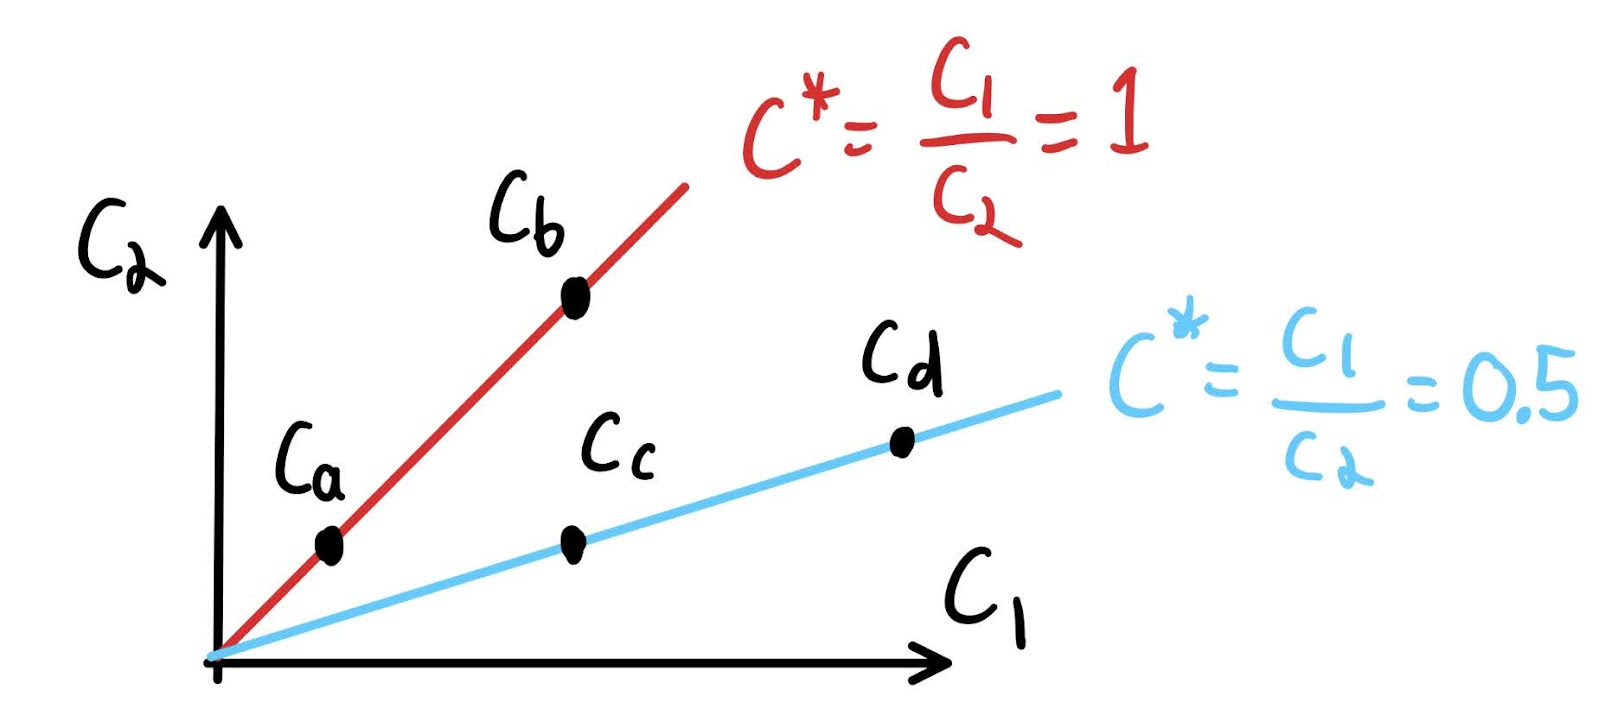
\includegraphics[width=0.80\linewidth]{fig/c_space2.jpg}
\caption{Dimensionally similar contexts example with dimensions: $m=2$ and $d=1$: $c_a$ is dimensionally similar to $c_b$ but not to $c_c$ or $c_d$.}\label{fig:c_space}
\end{center}
\vspace{-15pt}
\end{figure}
%%%%%%%%%%%%%%%%%%%%%%

For a given motion control problem, if the dimensionless context are equal, then the dimensionless feedback law should be exactly equivalent:
%%%%%%%%%%%%%%%%%%%%%%
\begin{equation}
\text{if} \quad c_a^* = c_b^*  \quad \text{then} \quad f_a^*(x^*) = f_b^*(x^*) \; \forall x^*   
\end{equation}
%%%%%%%%%%%%%%%%%%%%%%
where dimensionless feedback laws are defined as slices of the dimensionless policy for specific contexts:
%%%%%%%%%%%%%%%%%%%%%%
\begin{align}
f_a^*(x^*) = \pi^*( x^* , c^* = c_a^*)\\
f_b^*(x^*) = \pi^*( x^* , c^* = c_b^*)
\end{align}
%%%%%%%%%%%%%%%%%%%%%%
This is simply based on the fact that the dimensionless policy, i.e. eq. \eqref{eq:vectordimpolicyshort}, gives the same outputs for the same inputs. This results means that the knowledge of the policy for a specific context $c$ can actually be generalized to a sub-space of all context for which the dimensionless context $c^*$ is equal. For instance, lets imagine we have a global policy for a spherical submarine that depends only on the velocity and the radius. In dimensionless form we would find the policy depends only on the Reynolds number, thus would be equivalent for all pair of velocity and radius that correspond to the same Reynolds number.

\subsection{Transferring policies between contexts}

In order to exploit this property, it is useful to define transformation matrices based on scalar equations \eqref{eq:piu}, \eqref{eq:pix} and \eqref{eq:pic}:
%%%%%%%%%%%%%%%%%%%%%%
\begin{align}
u^* &= \left[ T_u(c) \right] \, u  \label{eq:Tu} \\
x^* &= \left[ T_x(c) \right] \, x \label{eq:Tx} \\
c^* &= \left[ T_c(c) \right] \, c \label{eq:Tc}
\end{align}
%%%%%%%%%%%%%%%%%%%%%%
where matrices $T_u$ and $T_x$ are square diagonal matrix, where each diagonal term is a multiplication of the first $d$ context variables ($\{c_1, c_2 , \hdots,c_d\}$) up to a rational power (found by applying the Buckingham $\pi$ theorem). Equations \eqref{eq:Tu} and \eqref{eq:Tx} are inversible (unless a context variable is equal to zero) and can be used to go back-and-forth between dimensional and dimensionless states and inputs variables. The matrix $T_c$ however have $d$ less row than columns and eq. \eqref{eq:Tc} is not inversible: for a given context $c$ there is only one dimensionless context $c^*$, however a dimensionless context $c^*$ correspond to multiple dimensional context $c$.

Using the transformation matrices, if a dimensional feedback law $f_a$ for a context $c_a$ is known:
%%%%%%%%%%%%%%%%%%%%%%
\begin{align}
f_a ( x ) &= \pi \left( x, c = c_a \right)
\end{align}
%%%%%%%%%%%%%%%%%%%%%%
its representation in dimensionless form:
%%%%%%%%%%%%%%%%%%%%%%
\begin{align}
f_a^* ( x^* ) &= \pi \left( x^*, c^* = c_a^* )\right) 
\end{align}
%%%%%%%%%%%%%%%%%%%%%%
can be found by scaling the input and output of $f_a$ with $T_u$ and $T_x$:
%%%%%%%%%%%%%%%%%%%%%%
\begin{align}
f_a^* ( x^* ) &= T_u(c_a) 
\underbrace{
f_a \left(  
\underbrace{
T_x^{-1}(c_a) \; x^*
}_{x}
\right)
}_{u}
\label{eq:f2star}
\end{align}
%%%%%%%%%%%%%%%%%%%%%%
Inversely, if we know a dimensionless feedback law $f_b^*$, matrices $T_u$ and $T_x$ can be used to scale it back to a specific context $c_b$:
%%%%%%%%%%%%%%%%%%%%%%
\begin{align}
f_b ( x ) &= T^{-1}_u(c_b) 
\underbrace{
f_b^* \left(  
\underbrace{
T_x(c_b) \; x
}_{x^*}
\right)
}_{u^*}
\label{eq:star2f}
\end{align}
%%%%%%%%%%%%%%%%%%%%%%
Thus, eq. \eqref{eq:f2star} and eq. \eqref{eq:star2f} can be used to take any context specific feedback law, finding its dimensionless form, and scale it back to a new context, as illustrated at Fig. \ref{fig:dimpol}. In general, there is no guarantee that the behaviour of the scaled feedback law in the new context will be similar to the behaviour of the feedback law in the original context, only if the context are dimensionally similar, i.e. the dimensionless context $c^*$ are equal. 
%%%%%%%%%%%%%%%%%%%%%%
\begin{figure}[htb]
\vspace{-5pt}
\begin{center}
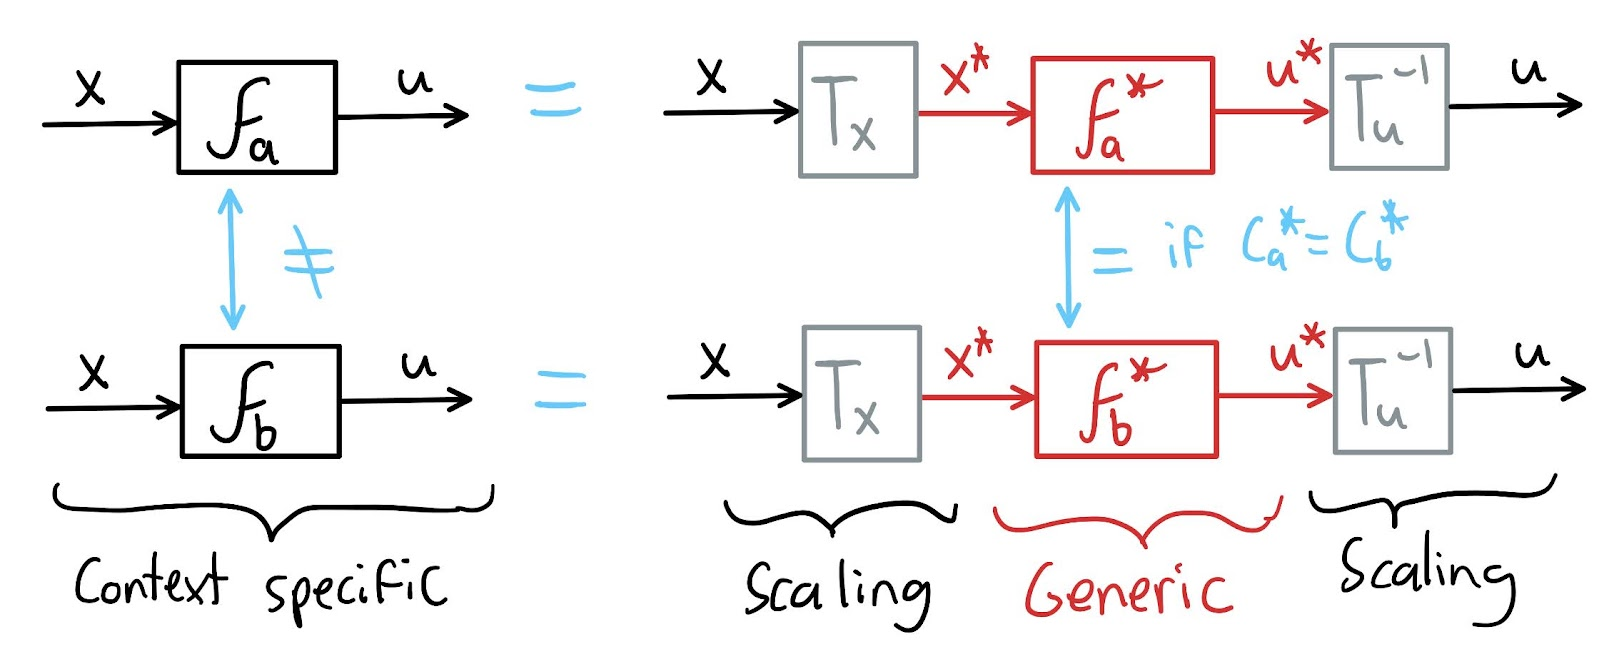
\includegraphics[width=0.99\linewidth]{fig/dimpol2.jpg}
\caption{Isolating the dimensionless knowledge in a policy}\label{fig:dimpol}
\end{center}
\vspace{-15pt}
\end{figure}
%%%%%%%%%%%%%%%%%%%%%%

Lets suppose an optimal policy solution $f_a$ is known for a specific context $c_a$, then the scaled policy:
%%%%%%%%%%%%%%%%%%%%%%
\begin{align}
f_b ( x ) &= 
\left[ T^{-1}_u(c_b) 
T_u(c_a) \right] \,
f_a \left( 
\left[
T_x^{-1}(c_a) 
T_x(c_b)
\right] \,
x
\right)
\label{eq:ab_transform}
\end{align}
%%%%%%%%%%%%%%%%%%%%%%
will be the optimal solution to the same motion control problem for a context $c_b$ if 
%%%%%%%%%%%%%%%%%%%%%%
\begin{equation}
c_b^* =  T_c( c_b ) \; c_b  = T_c( c_a ) \; c_a = c_a^* 
\label{eq:dimcontextequal}
\end{equation}
%%%%%%%%%%%%%%%%%%%%%%
In some sense, this similar context condition means that the motion problem with parameters $c_a$ and the motion problem with parameter $c_b$ were actually the exact same problem up to scaling factors. It thus make sense that the two solutions should thus also be equivalent up to scaling factors. 

In section \ref{sec:optimalswingup}, we show examples of this result with numerical solution to dimensionally similar pendulum swing-up problems. Furthermore, we demonstrate that in some situations, eq. \eqref{eq:dimcontextequal} equality conditions can be relaxed into inequality conditions, using the concept of regimes.



%%%%%%%%%%%%%%%%%%%%%%
\section{Optimal pendulum swing-up task}
\label{sec:optimalswingup}
In this paper, we will use the classical pendulum swing-up task to test the ideas of dimensionless policies. The motion control problem is formally defined here as finding a feedback law for controlling the dynamic system described by the differential equation:
%%%%%%%%%%%%%%%%%%%%%%
\begin{equation}
ml^2 \ddot{\theta} - mgl \sin \theta = \tau
\label{eq:pendulum_dynamics}
\end{equation}
%%%%%%%%%%%%%%%%%%%%%%
that minimize the quadratic cost function given by:
%%%%%%%%%%%%%%%%%%%%%%
\begin{equation}
J = \int{( q^2 \theta^2 + 0 \, \dot{\theta}^2 + 1 \, \tau^2 ) dt }
\label{eq:pendulum_cost}
\end{equation}
%%%%%%%%%%%%%%%%%%%%%%
subject to input constraints given by:
%%%%%%%%%%%%%%%%%%%%%%
\begin{equation}
- \tau_{max} \leq \tau \leq \tau_{max}
\label{eq:pendulum_constraints}
\end{equation}
%%%%%%%%%%%%%%%%%%%%%%
Note that here, 1) the cost function parameter $q$ is included with a power of two to have units of torque, 2) it was chosen to set to zero the weight on velocity for simplicity, and 3) the weight multiplying the torque is set to one without loss of generality as only the relative values of weights will impact the optimal solution. 

Thus, assuming there is no hidden variables and that equations \eqref{eq:pendulum_dynamics}, \eqref{eq:pendulum_cost} and \eqref{eq:pendulum_constraints} fully describe the problem. The solution, i.e. the optimal policy for all context, should be of the form given by:
%%%%%%%%%%%%%%%%%%%%%%
\begin{equation}
\underbrace{\tau}_{\text{inputs}}
=
\pi \left(
\underbrace{ \theta, \dot{\theta} }_{\text{states}},
\underbrace{
\underbrace{ m , g , l }_{\text{system parameters}},
\underbrace{ q , \tau_{max} }_{\text{task parameters}}
}_{\text{Context $c$}}
\right)
\end{equation}
%%%%%%%%%%%%%%%%%%%%%%
involving variables listed in table \ref{tb:optimalswingup}.
%%%%%%%%%%%%%%%%%%%%%%%%%%%%%%%%%%%%%%%%%%%%
\begin{table}[htb]
   \centering % center the table
   \caption{Pendulum swing-up optimal policy variables} 
   \label{tb:optimalswingup}
   \begin{tabular}{p{0.8cm} p{2.5cm} p{0.8cm} p{1.5cm} }
   \hline \hline \noalign{\smallskip} \noalign{\smallskip} \noalign{\smallskip} \noalign{\smallskip}
   %%%%%%%%%%%%%%%%%%%%%%
   \textbf{Variable} & \textbf{Description} & \textbf{Units} & \textbf{Dimensions} \\ 
   %%%%%%%%%%%%%%%%%%%%%%
   \hline \hline \noalign{\smallskip} 
   \multicolumn{4}{c}{\textbf{Control inputs}}\\ \noalign{\smallskip}  \hline \hline
   \noalign{\smallskip} 
   %%%%%%%%%%%%%%%%%%%%%%
   $\tau$ & Actuator torque & $Nm$ & [$ML^2T^{-2}$]\\ 
   %%%%%%%%%%%%%%%%%%%%%%
   \hline \hline \noalign{\smallskip} 
   \multicolumn{4}{c}{\textbf{State variables}}\\ \noalign{\smallskip}  \hline \hline \noalign{\smallskip} 
   %%%%%%%%%%%%%%%%%%%%%%
   $\theta$ & Joint angle & $rad$ & []\\ \noalign{\smallskip} \hline \noalign{\smallskip}
   $\dot{\theta}$ & Joint angular velocity & $rad/sec$ & [$T^{-1}$] \\
   %%%%%%%%%%%%%%%%%%%%%%
   \hline \hline \noalign{\smallskip} 
   \multicolumn{4}{c}{\textbf{System parameters}}\\ \noalign{\smallskip}  \hline\hline  \noalign{\smallskip} 
   %%%%%%%%%%%%%%%%%%%%%%
   $m$ & Pendulum mass & $kg$ & [$M$]  \\ \noalign{\smallskip} \hline \noalign{\smallskip}
   $g$ & Gravity       & $m/s^2$ & [$LT^{-2}$]  \\ \noalign{\smallskip} \hline \noalign{\smallskip}
   $l$ & Pendulum lenght & $m$ & [$L$]  \\ \noalign{\smallskip} \hline \noalign{\smallskip}
%%%%%%%%%%%%%%%%%%%%%%
   \hline \hline \noalign{\smallskip} 
   \multicolumn{4}{c}{\textbf{Problem parameters}}\\ \noalign{\smallskip}  \hline\hline  \noalign{\smallskip} 
   %%%%%%%%%%%%%%%%%%%%%%
   $q$ & Weight parameter  & $Nm$ & [$ML^2T^{-2}$]   \\ \noalign{\smallskip} \hline \noalign{\smallskip}
   $\tau_{max}$ & Maximum torque & $Nm$ & [$ML^2T^{-2}$] \\ \noalign{\smallskip} \hline \noalign{\smallskip}
   \hline \noalign{\smallskip}
   %\bottomrule[\heavyrulewidth] 
   \end{tabular}
\end{table}
%%%%%%%%%%%%%%%%%%%%%%%%%%%%%%%%%%%%%%%%%%%%

Before, conducting the dimensional analysis, it is interesting to note that while there are 3 system parameters $m$, $g$ and $l$, they only appear independently in two groups in the dynamic equation. We can thus consider only two system parameters. For convenience we selected $mgl$, corresponding to the maximum static gravitational torque (i.e. when the pendulum is horizontal) and $\omega$, as listed at table \ref{tb:2param}
%%%%%%%%%%%%%%%%%%%%%%%%%%%%%%%%%%%%%%%%%%%%
\begin{table}[htb]
   \centering % center the table
   \caption{Pendulum system parameters} 
   \label{tb:2param}
   \begin{tabular}{p{1.5cm} p{2.2cm} p{0.8cm} p{1.5cm} }
   \hline \hline \noalign{\smallskip} \noalign{\smallskip} 
   \textbf{Variable} & \textbf{Description} & \textbf{Units} & \textbf{Dimensions} \\ \noalign{\smallskip}  \hline\hline  \noalign{\smallskip} 
   %%%%%%%%%%%%%%%%%%%%%%
   $mgl$ & Maximum gravitational torque  & $Nm$ & [$ML^2T^{-2}$]  \\ \noalign{\smallskip} \hline \noalign{\smallskip}
   $\omega = \sqrt{\frac{g}{l}}$ & Natural frequency & $sec^{-1}$ & [$T^{-1}$]  \\ \noalign{\smallskip} \hline \noalign{\smallskip}
   \hline \noalign{\smallskip}
   %\bottomrule[\heavyrulewidth] 
   \end{tabular}
\end{table}
%%%%%%%%%%%%%%%%%%%%%%%%%%%%%%%%%%%%%%%%%%%%



% %%%%%%%%%%%%%%%%%%%%%%%%%%%%%%%%%%%%%%%%%%%%
% \subsection{Dimensionless dynamics}



% %%%%%%%%%%%%%%%%%%%%%%
% \begin{align}
% %ml^2 \ddot{\theta} + mgl \sin \theta &= \tau  \\
% \frac{\ddot{\theta}}{\omega^2} + \sin \theta &= \frac{\tau}{mgl}
% \end{align}
% %%%%%%%%%%%%%%%%%%%%%%

% %%%%%%%%%%%%%%%%%%%%%%
% \begin{equation}
% m = (n = 5 ) - ( p = 2 ) = 3
% \end{equation}
% %%%%%%%%%%%%%%%%%%%%%%

% %%%%%%%%%%%%%%%%%%%%%%
% \begin{align}
% \Pi_1 &= \tau^* = \frac{\tau}{mgl} \quad \quad \frac{[ML^2T^{-2}]}{[M][LT^{-2}][L]} \\
% \Pi_2 &= \theta^* = \theta \quad \quad [-]\\
% \Pi_3 &= \ddot{\theta}^* = \frac{ \ddot{\theta}  }{ \omega^2 } \quad \quad \frac{[T^{-2}]}{[T^{-1}][T^{-1}]} 
% \end{align}
% %%%%%%%%%%%%%%%%%%%%%%

% %%%%%%%%%%%%%%%%%%%%%%
% \begin{equation}
% \tau^*
% =
% f\left(
% \theta^*,\ddot{\theta}^*
% \right) = \ddot{\theta}^* + \sin \theta^*
% \end{equation}
% %%%%%%%%%%%%%%%%%%%%%%


\subsection{Dimensional analysis}

Here we have one control input, two states, two system parameters and two task parameters, for a total of $1+(n=2)+(m=4)=7$ variables are involved. In those variables, only $d=2$ independents dimensions ( $ML^2T^{-2}$ and $T^{-1}$ ) are present. Using $c_1 = mgl$ and $c_2 = \omega$ as the repeating variables leads to the following dimensionless groups:
%%%%%%%%%%%%%%%%%%%%%%
\begin{align}
\Pi_1 &= \tau^* = \frac{\tau}{mgl} \quad \quad \frac{[ML^2T^{-2}]}{[M][LT^{-2}][L]} \\
\Pi_2 &= \theta^* = \theta \quad \quad []\\
\Pi_3 &= \dot{\theta}^* = \frac{ \dot{\theta}  }{ \omega } \quad \quad \frac{[T^{-1}]}{[T^{-1}]} \\
\Pi_4 &= \tau_{max}^* = \frac{\tau_{max}}{mgl} \quad \quad \frac{[ML^2T^{-2}]}{[M][LT^{-2}][L]} \\
\Pi_5 &= q^* = \frac{q}{mgl} \quad \quad \frac{[ML^2T^{-2}]}{[M][LT^{-2}][L]} 
\end{align}
%%%%%%%%%%%%%%%%%%%%%%
All 3 torque variables ($\tau$, $q$ and $\tau_{max}$) are scaled by the maximum gravitational torque, and the pendulum velocity variable is scaled by the pendulum natural frequency. The transformation matrices are then:
%%%%%%%%%%%%%%%%%%%%%%
\begin{align}
\tau^* &= 
\underbrace{\left[  1/mgl \right]}_{T_u}
\, \tau  \label{eq:Tupendulum} \\
\begin{bmatrix}
\theta^* \\ \dot{\theta}^*
\end{bmatrix} &= 
\underbrace{
\begin{bmatrix}
    1 & 0 \\ 0 & 1/\omega
\end{bmatrix}
}_{T_x} \, 
\begin{bmatrix}
\theta \\ \dot{\theta}
\end{bmatrix}
 \label{eq:Txpendulum} \\
\underbrace{
\begin{bmatrix}
q^* \\ \tau_{max}^*
\end{bmatrix} 
}_{c^*} 
&= 
\underbrace{
\begin{bmatrix}
 0 & 0  & 1/mgl & 0 \\  0 & 0  & 0 &  1/mgl
\end{bmatrix}
}_{T_c} \, 
\underbrace{
\begin{bmatrix}
mgl \\ \omega \\ q \\ \tau_{max}
\end{bmatrix}
}_{c} 
 \label{eq:Tcpendulum} 
\end{align}
%%%%%%%%%%%%%%%%%%%%%%
According to the theorem, any policy that is only based on the variable included in our analysis can be restated as a relationship between the 5 dimensionless $\Pi$ groups:
%%%%%%%%%%%%%%%%%%%%%%
\begin{equation}
\tau^*
=
\pi^* \left(
\theta, \dot{\theta}^*,
q^* , \tau_{max}^* 
\right)
\end{equation}
%%%%%%%%%%%%%%%%%%%%%%

The dimensional analysis conducted at sec. \ref{sec:dimenanalysis}) told us that, for dimensionally similar swing-up problem (which means here equal ratios $q^*$ and $\tau_{max}^*$) the optimal feedback laws should be equivalent in their dimensionless form. In other words, if we have an optimal policy $f_a$ found in a specific context $c_a = [m_a,l_a,g_a,q_a,\tau_{max,a}]$, and an optimal policy $f_b$ for a second context $c_b = [m_b,l_b,g_b,q_b,\tau_{max,b}]$. Then, both dimensionless form will be equal $f_a^*=f_b^*$ if $q^*_a = q^*_b$ and $\tau_{max,a}^* = \tau_{max,b}^*$. Furthermore, we can thus find $f_b$ using $f_a$ or vice-versa using the scaling formula given by eq. \eqref{eq:ab_transform} if this condition is met. However, if $q^*_a \neq q^*_b$ or $\tau_{max,a}^* \neq \tau_{max,b}^*$ then $f_a$ doesn't give us information on $f_b$ without additional assumptions. 

%%%%%%%%%%%%%%%%%%%%%%
\subsection{Numerical results}
Here, we use a numerical algorithm (we give the details of the methodology at section \ref{sec:metho}) to compute numerical solutions to the motion control problem defined by eq \eqref{eq:pendulum_dynamics}, \eqref{eq:pendulum_cost} and \eqref{eq:pendulum_constraints}. The used numerical recipe produce feedback laws in the form of look-up tables, based on a discretized grid of the state-space.  The optimal (up to discretization errors) feedback laws are computed for 9 contexts listed at table \ref{tb:9contexts}. In those 9 contexts, there are 3 sub-groups of 3 with dimensionally similar contexts. Also each sub-group inlcudes the same 3 pendulums, illustrated at Fig. \ref{fig:big_picture}, a regular, a twice longer and a twice heavier. Contexts 1, 2 and 3 describe a task where the torque is limited to half the static maximum torque.  Contexts 4, 5 and 6 describe a task where the cost highly penalize applying large torques. Contexts 7, 8 and 9 describe a task where the cost highly penalize position errors. 
%%%%%%%%%%%%%%%%%%%%%%%%%%%%%%%%%%%%%%%%%%%%
\begin{table}[htb]
   \centering % center the table
   \caption{Pendulum swing-up problems parameters} 
   \label{tb:9contexts}
   \begin{tabular}{ p{2.0cm} p{0.8cm} p{0.8cm} p{0.8cm} p{0.8cm} p{0.8cm} }
   \hline \hline \noalign{\smallskip} \noalign{\smallskip} 
   %%%%%%%%%%%%%%%%%%%%%%
      & $m$ & $g$ & $l$ & $q$ & $\tau_{max}$ \\ \hline
   %%%%%%%%%%%%%%%%%%%%%
   %%%%%%%%%%%%%%%%%%%%%%
   \hline \hline \noalign{\smallskip} 
   \multicolumn{6}{c}{\textbf{Problems with $\tau_{max}^* = 0.5$ and $q^* = 0.1$} }\\ \noalign{\smallskip}  \hline\hline  \noalign{\smallskip} 
   %%%%%%%%%%%%%%%%%%%%%%
   Context no 1 : & 1.0 & 10.0 & 1.0 & 1.0 & 5.0 \\
   Context no 2 : & 1.0 & 10.0 & 2.0 & 2.0 & 10.0 \\
   Context no 3 : & 2.0 & 10.0 & 1.0 & 2.0 & 10.0 \\
   %%%%%%%%%%%%%%%%%%%%%
   \hline \hline \noalign{\smallskip} 
   \multicolumn{6}{c}{\textbf{Problems with $\tau_{max}^* = 1.0$ and $q^* = 0.05$} }\\ \noalign{\smallskip}  \hline\hline  \noalign{\smallskip} 
   %%%%%%%%%%%%%%%%%%%%%%
   Context no 4 : & 1.0 & 10.0 & 1.0 & 0.5 & 10.0 \\
   Context no 5 : & 1.0 & 10.0 & 2.0 & 1.0 & 20.0 \\
   Context no 6 : & 2.0 & 10.0 & 1.0 & 1.0 & 20.0 \\
   %%%%%%%%%%%%%%%%%%%%%
   \hline \hline \noalign{\smallskip} 
   \multicolumn{6}{c}{\textbf{Problems with $\tau_{max}^* = 1.0$ and $q^* = 10$} }\\ \noalign{\smallskip}  \hline\hline  \noalign{\smallskip} 
   %%%%%%%%%%%%%%%%%%%%%%
   Context no 7 : & 1.0 & 10.0 & 1.0 & 100.0 & 10.0 \\
   Context no 8 : & 1.0 & 10.0 & 2.0 & 200.0 & 20.0 \\
   Context no 9 : & 2.0 & 10.0 & 1.0 & 200.0 & 20.0 \\
   %%%%%%%%%%%%%%%%%%%%%
   \hline \hline
   \end{tabular}
\end{table}
%%%%%%%%%%%%%%%%%%%%%%%%%%%%%%%%%%%%%%%%%%%%

Figures \ref{fig:c1} to \ref{fig:c9} illustrate that for each sub-group with equal dimensionless context, the dimensional feedback law generated numerically looks very similar. They are similar up to a scaling of their axis, if we neglect slight differences due to discretization errors. Furthermore, when we compute the dimensionless version of the feedback laws $f^*$, using eq. \eqref{eq:f2star}, the dimensionless version is actually equal within each similar sub-group. This was the expected results predicted by the dimensional analysis of section \ref{sec:dimenanalysis}.

%%%%%%%%%%%%%%%%%%%%%%%%%%%%
 \begin{figure*}[htp]
    \centering
    \vspace{-10pt}
    \subfloat[Feedback law $f$]{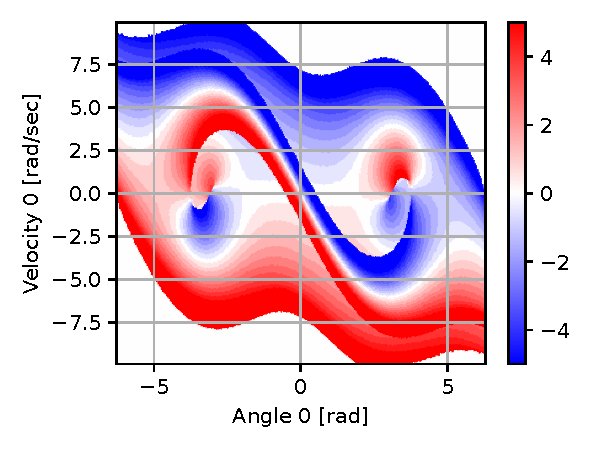
\includegraphics[width=0.33\textwidth]{fig/c1_policy.pdf}}
    \subfloat[Dimensionless feedback law $f^*$]{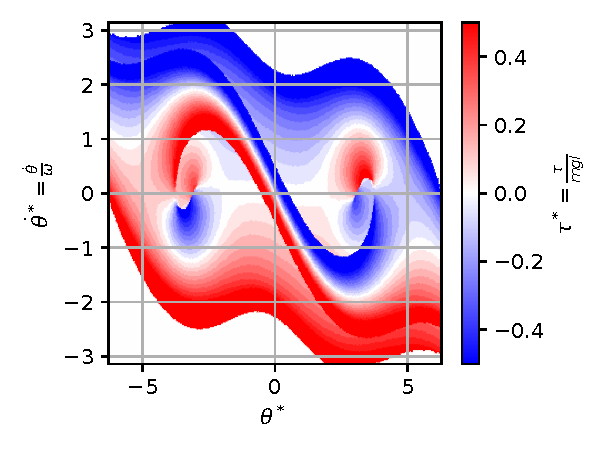
\includegraphics[width=0.33\textwidth]{fig/c1_dimpolicy.pdf}}   
    \subfloat[Optimal trajectory starting at $\theta=-\pi$]{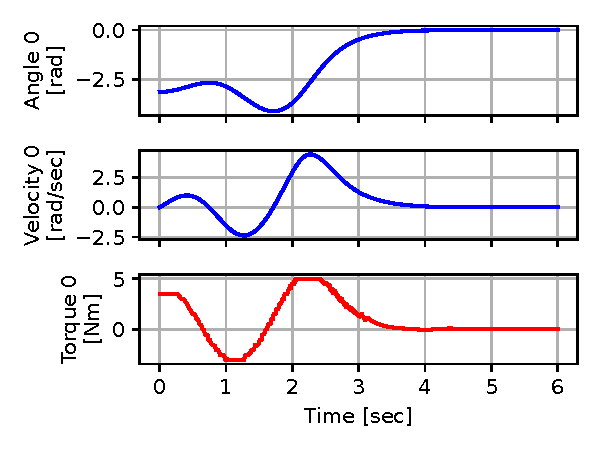
\includegraphics[width=0.33\textwidth]{fig/c1_traj.pdf}}
    \caption{Numerical results for context no 1}
    \label{fig:c1}
\end{figure*}
%%%%%%%%%%%%%%%%%%%%%%%%%%%%
 \begin{figure*}[htp]
    \centering
    \vspace{-10pt}
    \subfloat[Feedback law $f$]{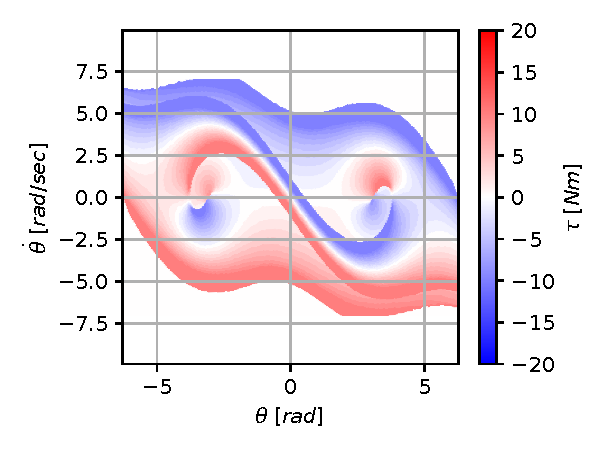
\includegraphics[width=0.33\textwidth]{fig/c2_policy.pdf}}
    \subfloat[Dimensionless feedback law $f^*$]{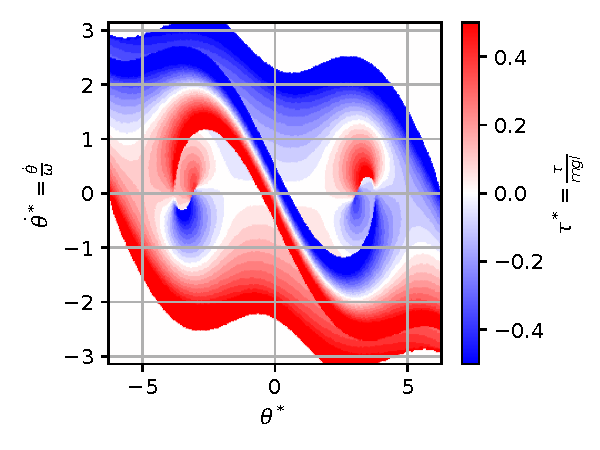
\includegraphics[width=0.33\textwidth]{fig/c2_dimpolicy.pdf}}   
    \subfloat[Optimal trajectory starting at $\theta=-\pi$]{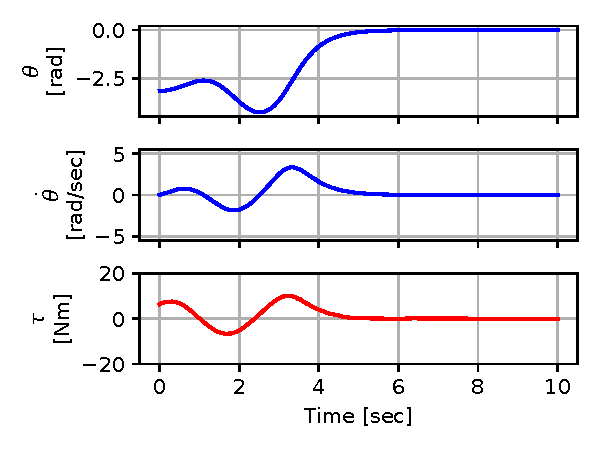
\includegraphics[width=0.33\textwidth]{fig/c2_traj.pdf}}
    \caption{Numerical results for context no 2}
    \label{fig:c2}
\end{figure*}
%%%%%%%%%%%%%%%%%%%%%%%%%%%%
 \begin{figure*}[htp]
    \centering
    \vspace{-10pt}
    \subfloat[Feedback law $f$]{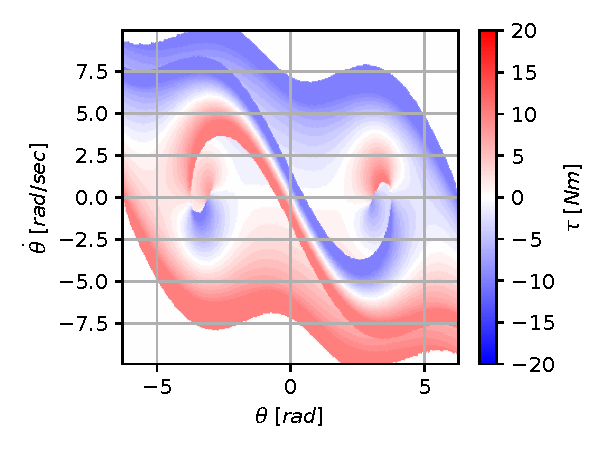
\includegraphics[width=0.33\textwidth]{fig/c3_policy.pdf}}
    \subfloat[Dimensionless feedback law $f^*$]{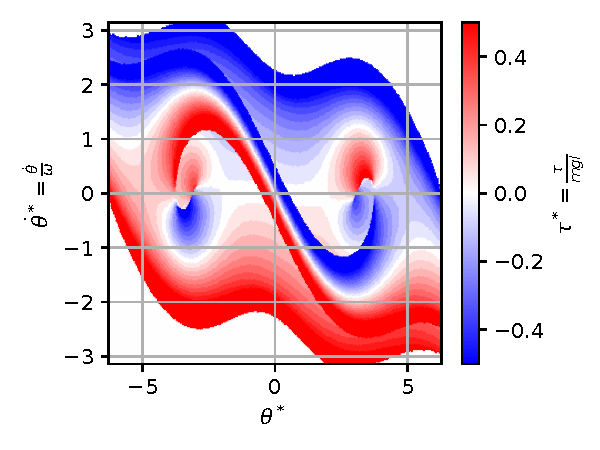
\includegraphics[width=0.33\textwidth]{fig/c3_dimpolicy.pdf}}   
    \subfloat[Optimal trajectory starting at $\theta=-\pi$]{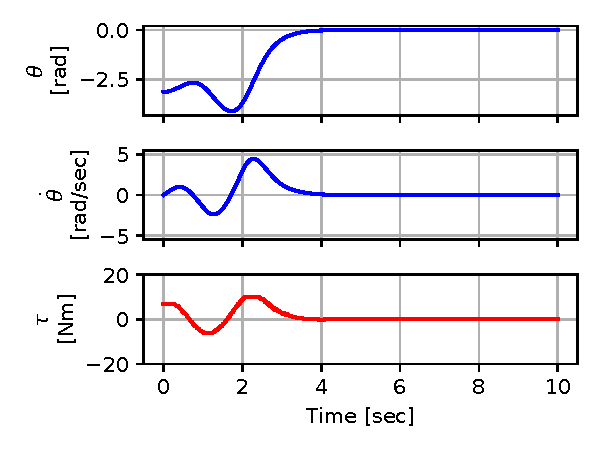
\includegraphics[width=0.33\textwidth]{fig/c3_traj.pdf}}
    \caption{Numerical results for context no 3}
    \label{fig:c3}
\end{figure*}
%%%%%%%%%%%%%%%%%%%%%%%%%%%%
 \begin{figure*}[htp]
    \centering
    \vspace{-10pt}
    \subfloat[Feedback law $f$]{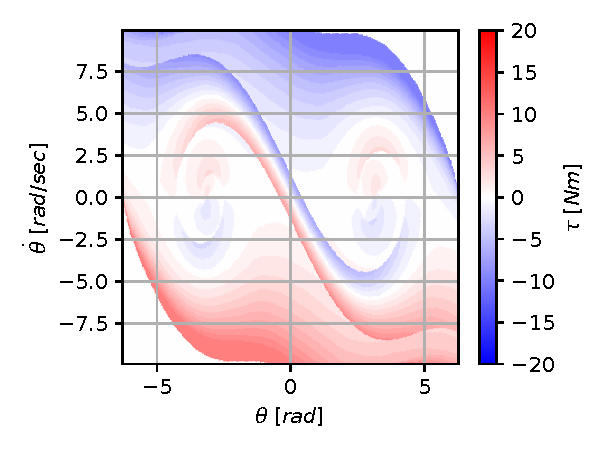
\includegraphics[width=0.33\textwidth]{fig/c4_policy.pdf}}
    \subfloat[Dimensionless feedback law $f^*$]{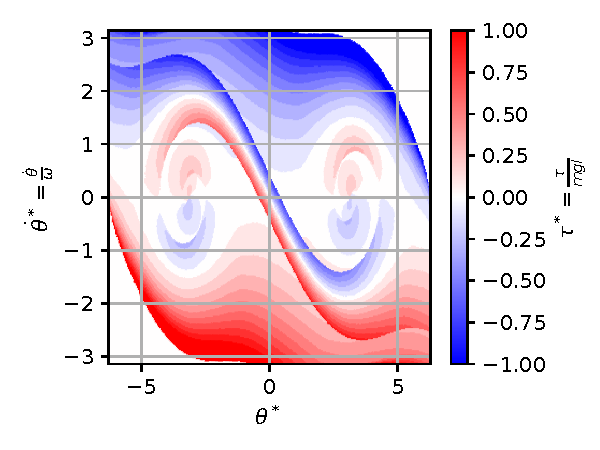
\includegraphics[width=0.33\textwidth]{fig/c4_dimpolicy.pdf}}   
    \subfloat[Optimal trajectory starting at $\theta=-\pi$]{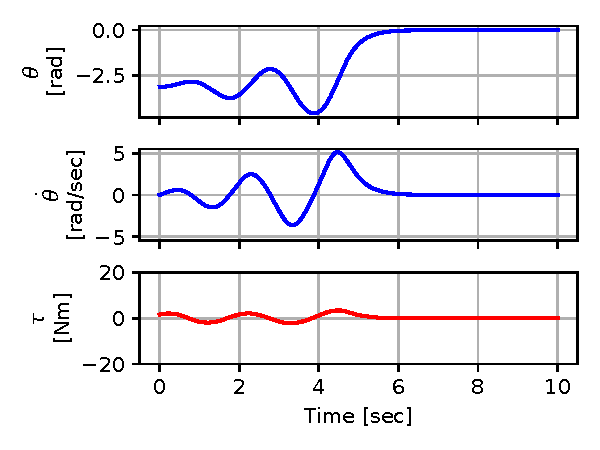
\includegraphics[width=0.33\textwidth]{fig/c4_traj.pdf}}
    \caption{Numerical results for context no 4}
    \label{fig:c4}
\end{figure*}
%%%%%%%%%%%%%%%%%%%%%%%%%%%%
 \begin{figure*}[htp]
    \centering
    \vspace{-10pt}
    \subfloat[Feedback law $f$]{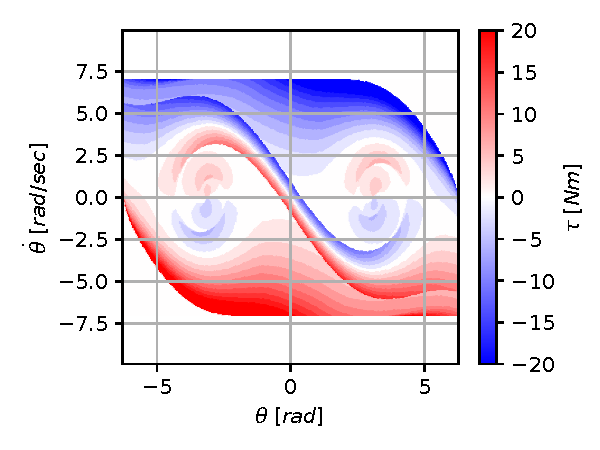
\includegraphics[width=0.33\textwidth]{fig/c5_policy.pdf}}
    \subfloat[Dimensionless feedback law $f^*$]{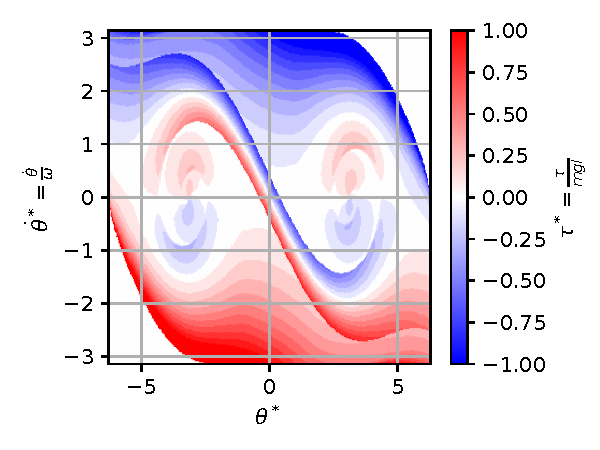
\includegraphics[width=0.33\textwidth]{fig/c5_dimpolicy.pdf}}   
    \subfloat[Optimal trajectory starting at $\theta=-\pi$]{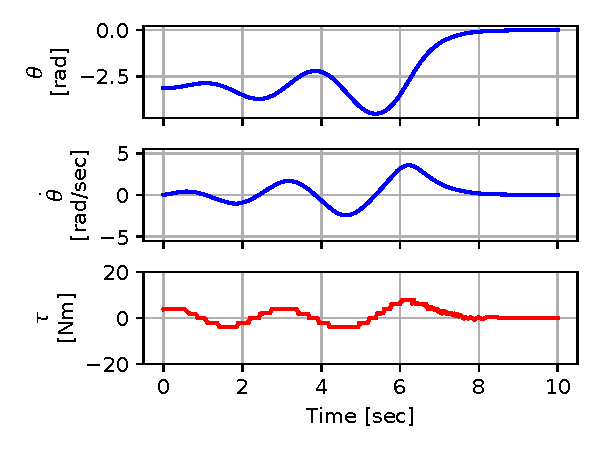
\includegraphics[width=0.33\textwidth]{fig/c5_traj.pdf}}
    \caption{Numerical results for context no 5}
    \label{fig:c5}
\end{figure*}
%%%%%%%%%%%%%%%%%%%%%%%%%%%%
 \begin{figure*}[htp]
    \centering
    \vspace{-10pt}
    \subfloat[Feedback law $f$]{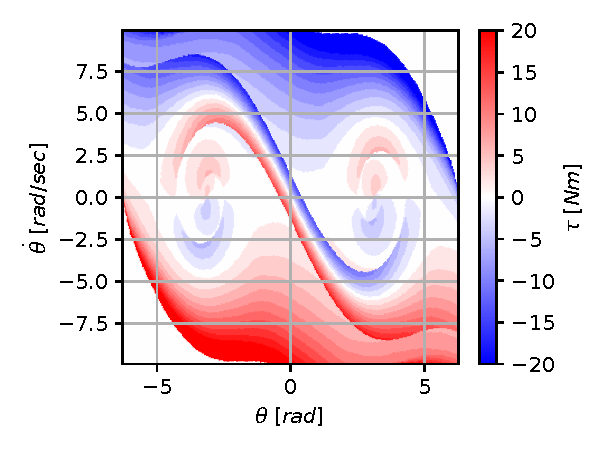
\includegraphics[width=0.33\textwidth]{fig/c6_policy.pdf}}
    \subfloat[Dimensionless feedback law $f^*$]{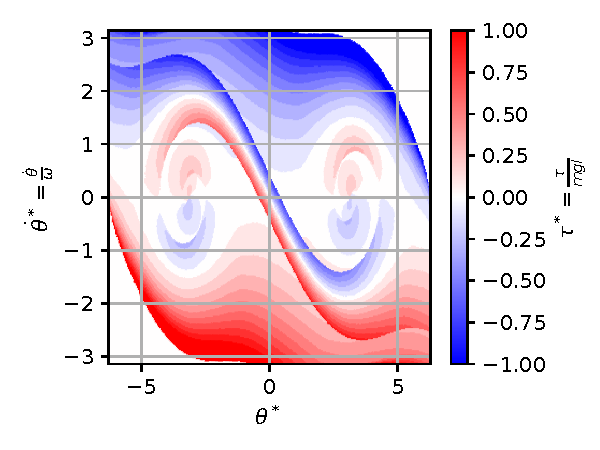
\includegraphics[width=0.33\textwidth]{fig/c6_dimpolicy.pdf}}   
    \subfloat[Optimal trajectory starting at $\theta=-\pi$]{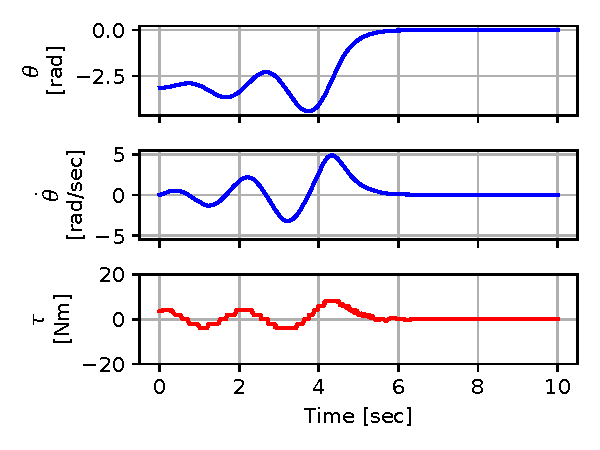
\includegraphics[width=0.33\textwidth]{fig/c6_traj.pdf}}
    \caption{Numerical results for context no 6}
    \label{fig:c6}
\end{figure*}
%%%%%%%%%%%%%%%%%%%%%%%%%%%%
 \begin{figure*}[htp]
    \centering
    \vspace{-10pt}
    \subfloat[Feedback law $f$]{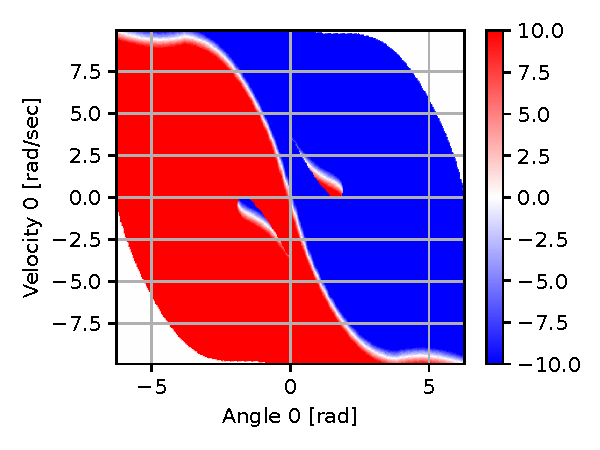
\includegraphics[width=0.33\textwidth]{fig/c7_policy.pdf}}
    \subfloat[Dimensionless feedback law $f^*$]{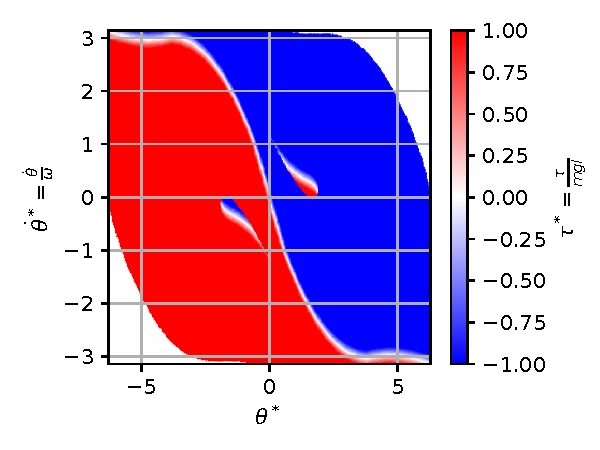
\includegraphics[width=0.33\textwidth]{fig/c7_dimpolicy.pdf}}   
    \subfloat[Optimal trajectory starting at $\theta=-\pi$]{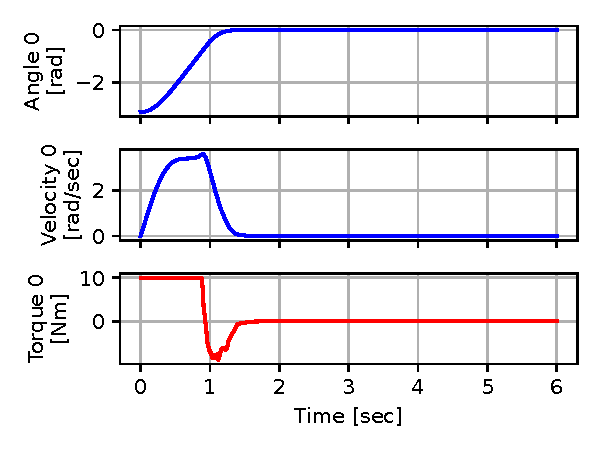
\includegraphics[width=0.33\textwidth]{fig/c7_traj.pdf}}
    \caption{Numerical results for context no 7}
    \label{fig:c7}
\end{figure*}
%%%%%%%%%%%%%%%%%%%%%%%%%%%%
 \begin{figure*}[htp]
    \centering
    \vspace{-10pt}
    \subfloat[Feedback law $f$]{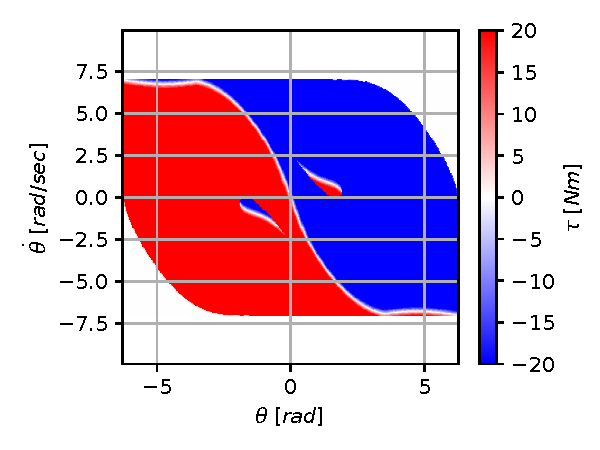
\includegraphics[width=0.33\textwidth]{fig/c8_policy.pdf}}
    \subfloat[Dimensionless feedback law $f^*$]{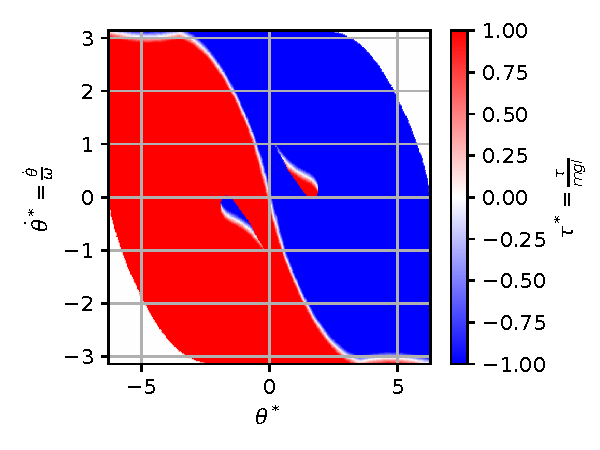
\includegraphics[width=0.33\textwidth]{fig/c8_dimpolicy.pdf}}   
    \subfloat[Optimal trajectory starting at $\theta=-\pi$]{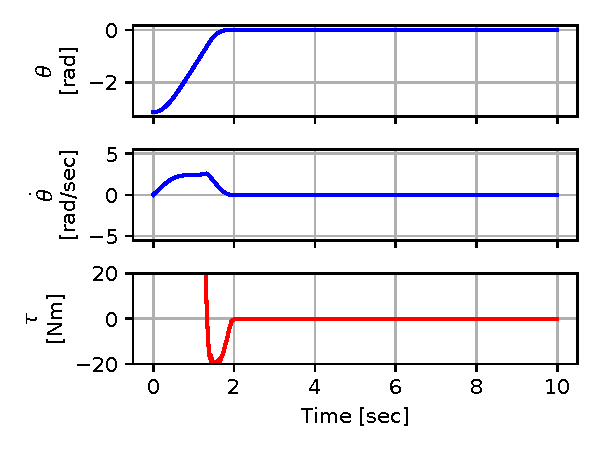
\includegraphics[width=0.33\textwidth]{fig/c8_traj.pdf}}
    \caption{Numerical results for context no 8}
    \label{fig:c8}
\end{figure*}
%%%%%%%%%%%%%%%%%%%%%%%%%%%%
 \begin{figure*}[htp]
    \centering
    \vspace{-10pt}
    \subfloat[Feedback law $f$]{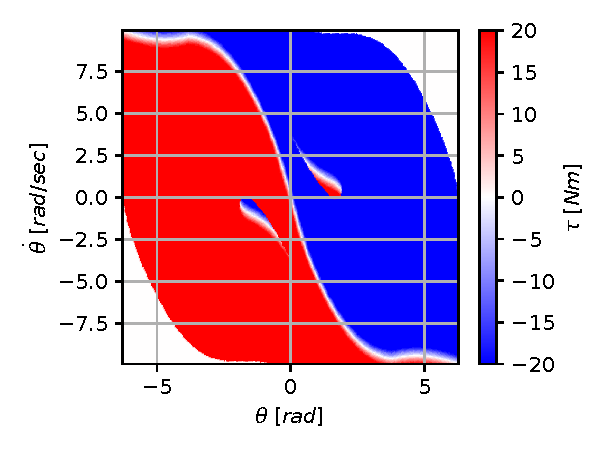
\includegraphics[width=0.33\textwidth]{fig/c9_policy.pdf}}
    \subfloat[Dimensionless feedback law $f^*$]{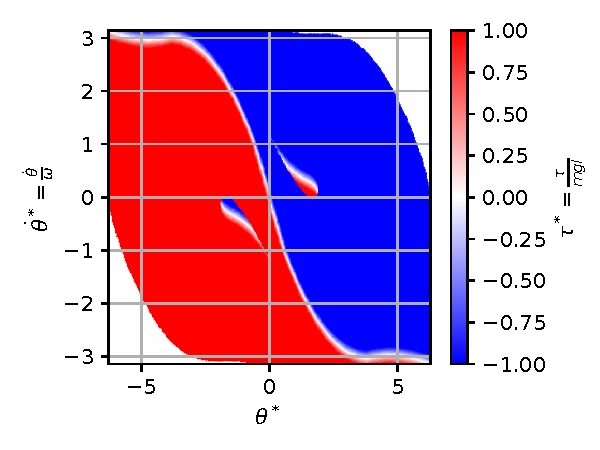
\includegraphics[width=0.33\textwidth]{fig/c9_dimpolicy.pdf}}   
    \subfloat[Optimal trajectory starting at $\theta=-\pi$]{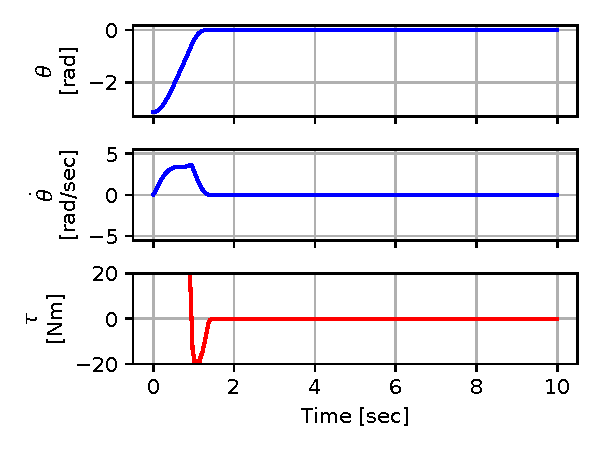
\includegraphics[width=0.33\textwidth]{fig/c9_traj.pdf}}
    \caption{Numerical results for context no 9}
    \label{fig:c9}
\end{figure*}
%%%%%%%%%%%%%%%%%%%%%%%%%%%%

In terms of how to use this in a practical scenario, we see that if we computed the feedback law given by Fig. \ref{fig:c1}(a), we can get the feedback law given by Fig. \ref{fig:c2}(a) or Fig. \ref{fig:c3}(a) directly by scaling the original policy with eq. \eqref{eq:ab_transform}, using the appropriate context variables, without having to recompute. In some sense, we got back the ability to adjust the feedback law on the fly to new system parameters $mgl$ or $\omega$, as it would be the case with an analytical solution. But this only works within the dimensionally similar context sub-group. The feedback law given by Fig. \ref{fig:c1}(a) cannot be scaled into the feedback law given by Fig. \ref{fig:c4}(a) or Fig. \ref{fig:c7}(a) for instance, since $\tau^*_{max}$ and $q^*$ are not equals. 

%%%%%%%%%%%%%%%%%%%%%%%%%%%%%%%%%%%%%%%%%%%%%%%%%%%
\subsection{Trajectory solutions}

Trajectory solutions are also generalizable in their dimensionless forms. Figures \ref{fig:c1}(c) to \ref{fig:c9}(c) show optimal trajectory solutions starting from the bottom position at rest. Those trajectories were computed by executing the computed optimal policies in a simulation. We can also see that within the 3 dimensionally similar sub-groups, the optimal trajectories are actually the same but scaled. Lets assume we were trying to solve a slightly different motion control problem. Instead of looking for feedback laws, lets assume we were looking for optimal trajectories. We must then think about this motion problem as looking for three time-based policies defining trajectories for states and inputs:
%%%%%%%%%%%%%%%%%%%%%%
\begin{align}
\tau          = \pi_{\tau}( t , &
 \, m , g , l , q , \tau_{max} )  \label{eq:traj_policy_1}\\
\theta        = \pi_{\theta}( t ,&
 \, m , g , l , q , \tau_{max} )
\label{eq:traj_policy_2}\\
\underbrace{
\dot{\theta } = \pi_{\dot{\theta }}( t 
 }_{\text{trajectory}} ,&
\underbrace{
m , g , l , q , \tau_{max} 
 }_{\text{context}} )
 \label{eq:traj_policy_3}
\end{align}
%%%%%%%%%%%%%%%%%%%%%%
Here, we can thus use the same dimensionless group as before, but with the addition of a dimensionless time:
%%%%%%%%%%%%%%%%%%%%%%
\begin{align}
t^* &= t \; \omega \quad \quad [T][T^{-1}]
\end{align}
%%%%%%%%%%%%%%%%%%%%%%
since the time $t$ is now explicitly an argument of the mappings. Applying the same dimensional analysis, to eq. \eqref{eq:traj_policy_1}, eq. \eqref{eq:traj_policy_2} and eq. \eqref{eq:traj_policy_3}, we would conclude that it can be restated as:
% %%%%%%%%%%%%%%%%%%%%%%
% \begin{align}
% \underbrace{
% \tau^*  = \pi_{\tau}^*( t^* 
% }_{\text{Dimensionless trajectory}} , 
% \underbrace{
% q^* , \tau_{max}^*
% }_{c^*} ) 
% \label{eq:dim_traj_policy}
% \end{align}
% %%%%%%%%%%%%%%%%%%%%%%
%%%%%%%%%%%%%%%%%%%%%%
\begin{align}
\tau^*          = \pi^*_{\tau}( t^* , &
 \, q^* , \tau_{max}^* )  \label{eq:dim_traj_policy_1}\\
\theta^*        = \pi^*_{\theta}( t^* ,&
 \, q^* , \tau_{max}^* )
\label{eq:dim_traj_policy_2}\\
\underbrace{
\dot{\theta }^* = \pi^*_{\dot{\theta }}( t^* 
}_{\text{dim. trajectory}} ,&
\underbrace{
 q^* , \tau_{max}^*
 }_{c^*} )
 \label{eq:dim_traj_policy_3}
\end{align}
%%%%%%%%%%%%%%%%%%%%%%
Hence, as it is the case for the feedback laws, the optimal trajectories should be equivalent in their dimensionless version, if the dimensionless context is equal. 



%%%%%%%%%%%%%%%%%%%%%%%%%%%%%%%%%%%%%%%%%%%%%%%%%%%
\subsection{Regimes of solutions}

In some situation, changing a context variable will not have any effect on the optimal policy. For instance, for the torque-limited optimal pendulum swing-up problem, augmenting $\tau_{max}$ or $q$ while keeping the other value fixed will have little effect pass a given threshold. If we look at the solutions for context no 4, 5 and 6, using a lot of torque is so highly penalized by the cost function that the saturation limit is not really impacting the solution (except edges cases on the boundary), hence we would expect that augmenting $\tau_{max}$ should not change the solution. 

Fig. \ref{fig:torque_sensitivity} and \ref{fig:q_sensitivity} show a slice (to allow visualization) of the optimal policy solution, for various contexts. Fig. \ref{fig:torque_sensitivity} illustrates changing $\tau_{max}^*$ while keeping $q^*$ fixed. We can see that when $\tau_{max}^*<0.3$ the policy is almost always on the min-max allowable values, this behaviour is often called \textit{bang-bang}. At the other extreme when 
$\tau_{max}^*>2.5$ the policy solution is continuous and almost never affected by the saturation. Fig. \ref{fig:q_sensitivity} illustrates changing $q^*$ while keeping $\tau_{max}^*$ fixed. We can see that when $q^*<0.1$ the optimal policy solution does not reach the min-max saturation, while when $q^*>1.0$, the policy is almost always on the min-max allowable values.% We can note that in the limit of very large $q^*$ value, the motion control problem would then to be equivalent to the minimum time problem, for which we know the solution is a bang-bang policy.
%%%%%%%%%%%%%%%%%%%%%%
\begin{figure}[ht]
\begin{center}
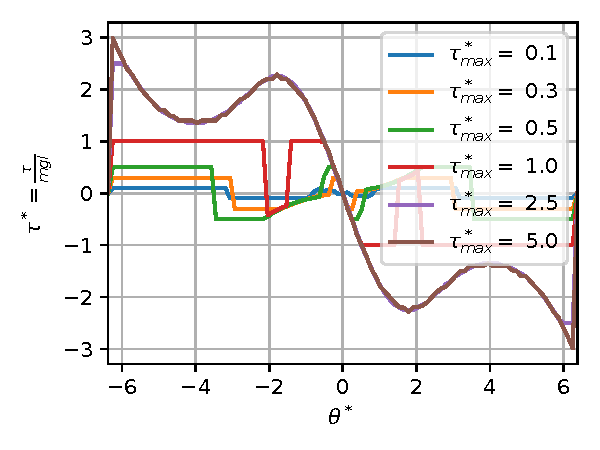
\includegraphics[width=0.99\linewidth]{fig/qs05.pdf}
\caption{Optimal dimensionless policy for various contexts $\tau^* = \pi^*( \theta^* , \dot{\theta}^* = 0 , q^* = 0.5 , \tau^*_{max} = [0.1, ... , 5.0] )$}
\vspace{-10pt}
\label{fig:torque_sensitivity}
\end{center}
\end{figure}
%%%%%%%%%%%%%%%%%%%%%%
%%%%%%%%%%%%%%%%%%%%%%
\begin{figure}[ht]
\begin{center}
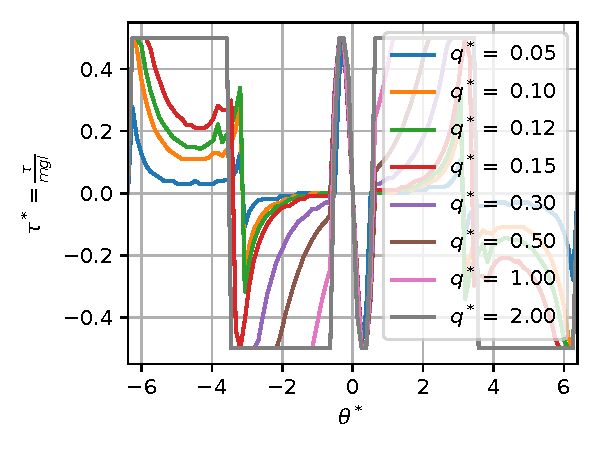
\includegraphics[width=0.99\linewidth]{fig/s_q_5_2.pdf}
\caption{Optimal dimensionless policy for various contexts  $\tau^* = \pi^*( \theta^*  , \dot{\theta}^* = 0 , q^* = [0.05, ... , 2.0]  , \tau^*_{max} = 0.5 )$}
\vspace{-10pt}
\label{fig:q_sensitivity}
\end{center}
\end{figure}
%%%%%%%%%%%%%%%%%%%%%%

We can see that for extreme context values, we have two type of behaviour, illustrated as region in the dimensionless context space at Fig. \ref{fig:regimeszones}. 
%%%%%%%%%%%%%%%%%%%%%%
\begin{figure}[ht]
\begin{center}
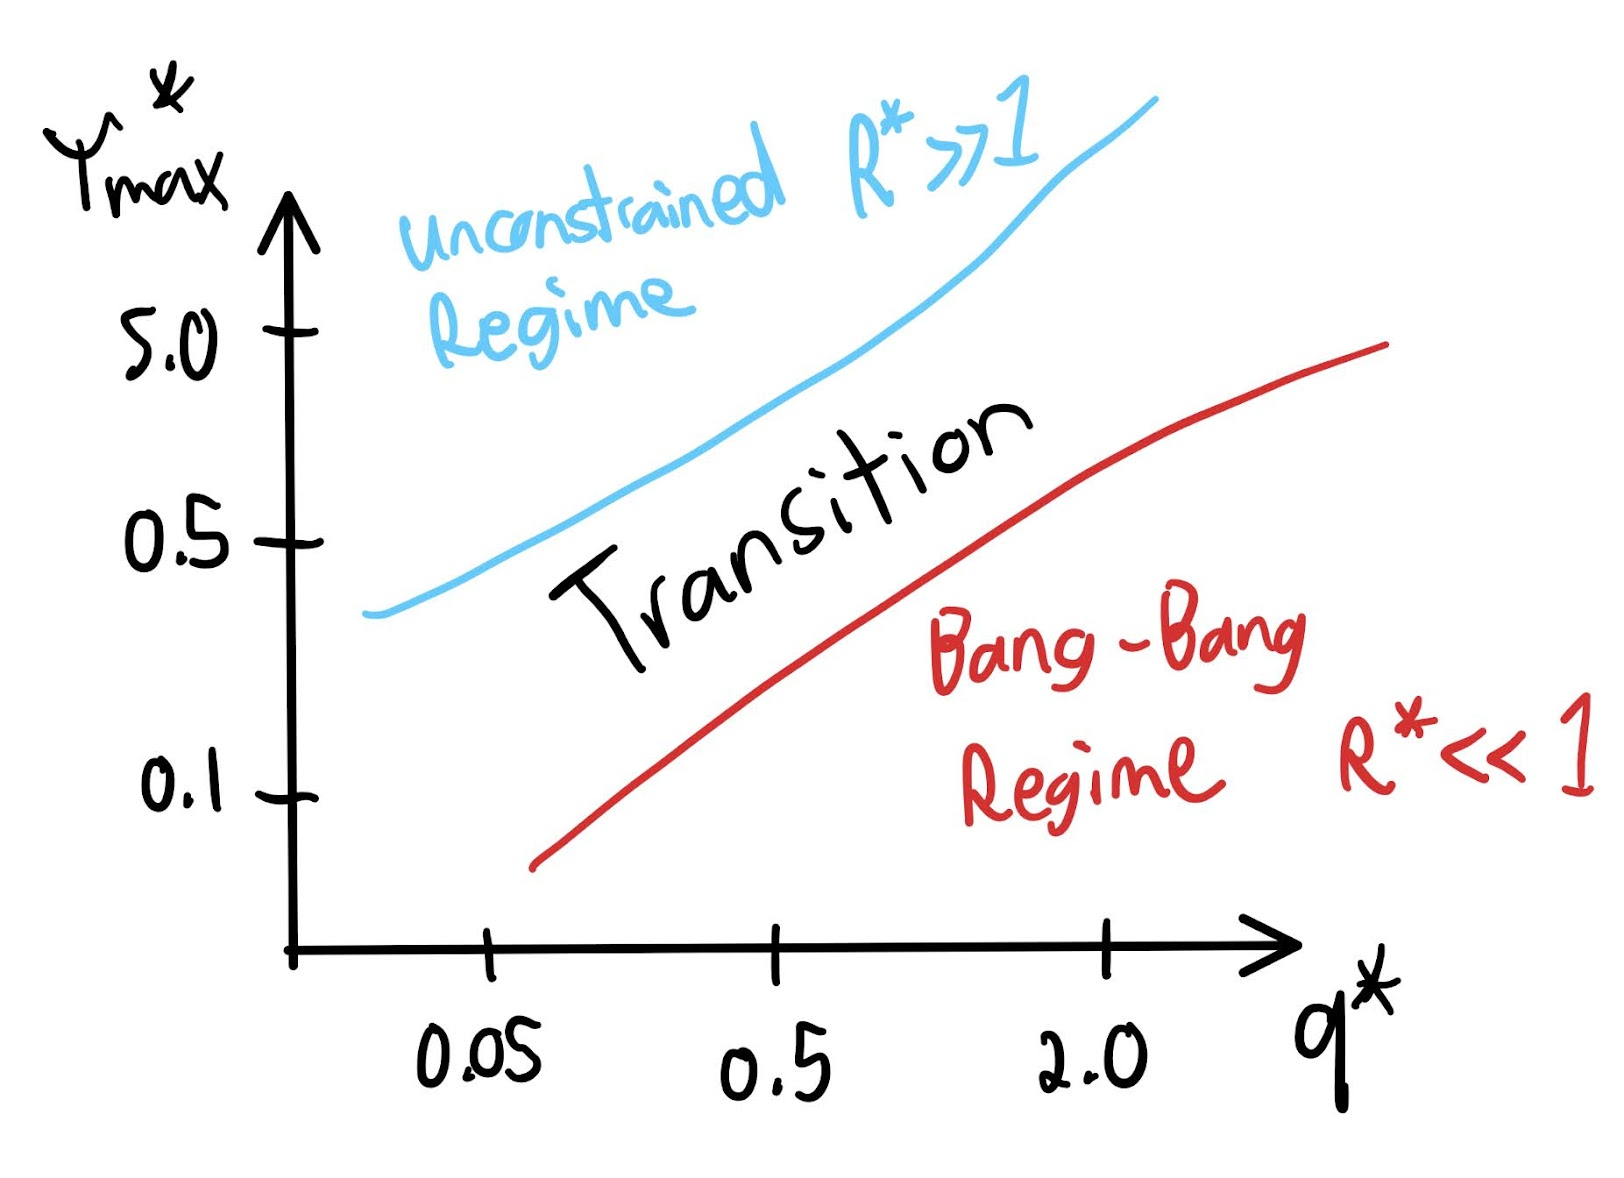
\includegraphics[width=0.99\linewidth]{fig/regime_zones2.jpg}
\caption{Regime zones}
\vspace{-10pt}
\label{fig:regimeszones}
\end{center}
\end{figure}
%%%%%%%%%%%%%%%%%%%%%%
Those regions are best caracterized by a ratio of $q^*$ and $\tau_{max}^*$, a new dimensionless value that we will define as the ratio of the maximum torque saturation $\tau_{max}$ over the weight in the cost function $q$:
%%%%%%%%%%%%%%%%%%%%%%
\begin{align}
R^* = \frac{\tau^*_{max}}{q^*} = \frac{\tau_{max}}{q} \quad\quad 
\end{align}
%%%%%%%%%%%%%%%%%%%%%%
When the value of $R^* \approx 1$, the policy solution is partially continuous, and on the min-max value in some other region of the state-space, a behaviour we will call the transition regime. When the value of $R^* \ll 1$, the constraint on torque drives the solution to have have a bang-bang type behaviour. In this region, that we would approximate here based on our sensitivity analysis to $R^* \ll 0.1$, the global policy is only a function of $\tau_{max}^*$:
%%%%%%%%%%%%%%%%%%%%%%
\begin{align}
\pi^*( \theta^* , \dot{\theta}^*, q^*, \tau_{max}^*) &\approx 
\pi^*( \theta^* , \dot{\theta}^* , \tau_{max}^* ) \; \text{if} \; R^* \ll 1
\label{eq:bangbang_policy}
\end{align}
%%%%%%%%%%%%%%%%%%%%%%
i.e. the value of $q^*$ is not affecting the solution. On the other hang, when the value of $R^* \gg 1$, the policy is unconstrained. In this region, that we would approximate here based on our sensitivity analysis to $R^* \gg 10$, the global policy is only a function of $q^*$ since the constraint is so far away:
%%%%%%%%%%%%%%%%%%%%%%
\begin{align}
\pi^*( \theta^* , \dot{\theta}^*, q^*, \tau_{max}^*) &\approx 
\pi^*( \theta^* , \dot{\theta}^* , q^* ) \; \text{if} \;  R^* \gg 1 
\label{eq:unconstrained_policy}
\end{align}
%%%%%%%%%%%%%%%%%%%%%%

The concept of regime is often leveraged in fluid mechanics, it allow to generalize results between situation where the relevant dimensionless number are not exactly matched. For instance, when the Mach number is small $Ma < 0.3$, we can generally assume to be in an incompressible regime where various speed of sound (for instance having $Ma=0.1$ or $Ma=0.3$) would not really change the behaviour. Here, for the purpose of transferring policy solution between contexts, it means that the condition of having the same exact dimensionless context variables can be relaxed with an inequality that correspond to a regime. For instance, for two motion control problems, if both context are in the unconstrained regime, it is sufficient to match only $q^*$ to have equivalent dimensionless policies. More formally, from eq. \eqref{eq:unconstrained_policy}, we can say that:
%%%%%%%%%%%%%%%%%%%%%%
\begin{align}
f_a^*(x^*) &= f_b^*(x^*) \;\forall\;  x^* 
\\ &\text{if} \quad q^*_a=q^*_b \; \text{,} \quad R^*_a \gg 1 \quad \text{and} \quad R^*_b \gg 1
\end{align}
%%%%%%%%%%%%%%%%%%%%%%
Also, for two motion control problems, if both context are in the bang-bang regime, it is sufficient to match only $\tau_{max}^*$ to have equivalent dimensionless policies. More formally, from eq. \eqref{eq:bangbang_policy}, we can say that:
%%%%%%%%%%%%%%%%%%%%%%
\begin{align}
f_a^*(x^*) &= f_b^*(x^*) \;\forall\;  x^* 
\\ &\text{if} \quad \tau_{max,a}^*=\tau_{max,b}^* \; \text{,} \; R^*_a \ll 1 \; \text{and} \; R^*_b \ll 1
\end{align}
%%%%%%%%%%%%%%%%%%%%%%
Another point of view, is that assuming we are in one of those regime means we could have removed one variable from the context from the start of the dimensional analysis. All in all, the impact of having such regimes identified is that we can increase the sub-space of contexts for which the dimensionless version of the policy should be equivalent, leading to a potentially larger pool of systems that can share learned policy or numerical results. 








\subsection{Methodology}
\label{sec:metho}

We obtained the optimal feedback law by using the basic dynamic programming algorithm \cite{bertsekas_dynamic_2012} on a discretized version of the continuous system. The approach is almost equivalent to the value iteration  algorithm \cite{sutton_reinforcement_2018}, sometime refer to as model-based reinforcement learning, with the exception that here the total number of iteration steps was  fixed (corresponding to a very long time horizon), instead of stopping the iteration after reaching a convergence criterion. This approach was chosen to have consistent results across all contexts, that lead to wide range of order-of-magnitude cost-to-go solution $J$. The selected discretization parameters are as follow:
the time step is 0.025 sec, the state space is discretized into an even 501 x 501 grid and the continuous torque is discretized into 101 discrete control options. Special out-of-bound and on-target termination states are included to
guarantee convergence \cite{bertsekas_dynamic_2012}. The source code is available here: \url{https://github.com/SherbyRobotics/pyro/blob/dimensionless/dev/dimensionless/cases_master.py} and this google colab page allow reproducing the results: \url{https://colab.research.google.com/drive/1kf3apyHlf5t7XzJ3uVM8mgDsneVK_63r?usp=sharing}.


\subsubsection{Additionnal dimensionless parameters for the solver}

Using dynamic programming for solving the optimal policy numerically required setting additional parameters that define the domain. Although those parameter should not affect the optimal policy far away from the boundaries, here a dimensionless version of those parameters was kept fixed in all the experiments:
%%%%%%%%%%%%%%%%%%%%%%
\begin{align}
\theta^*_{max} &= \theta_{max} = 2 \pi \\
\dot{\theta}^*_{max} &= \frac{ \dot{\theta}_{max} }{\omega} = \pi \\
t^*_{f} &= t_{f} \; \omega = 20 \times 2 \pi 
\end{align}
%%%%%%%%%%%%%%%%%%%%%%
where $\theta_{max}$ is the range of angles for witch the optimal policy is solved, here set at one full revolution, $\dot{\theta}_{max}$ is the range of angular velocity for witch the optimal policy is solved, and $t_{f}$ is the time horizon, set to 20 periods of the pendulum using the natural frequency.



%%%%%%%%%%%%%%%%%%%%%%%%%%%%%%%%%%%%%%%%%%%%%%%%%
\section{Closed-form parametric policies}
\label{sec:closedfrom}

To better understand the concept of a dimensionless policy, here we apply the Buckingham $\pi$ theorem on well-known closed form solution to classical motion control problems.


%%%%%%%%%%%%%%%%%%%%%%%%%%%%%%%%%%%%%%%%%%%%%%%%%%%%%%%
\subsection{ Dimensionless Linear Quatratic Reglator (LQR) solution}
\label{sec:lqr}

Here we analyse a simplified motion control problem with the LQR framework. A linearized verison of the equation of motion is used:
%%%%%%%%%%%%%%%%%%%%%%
\begin{equation}
ml^2 \ddot{\theta} - mgl \theta = \tau
\label{eq:pendulum_dynamics_lqr}
\end{equation}
%%%%%%%%%%%%%%%%%%%%%%
Also, the same cost function that was used in section \ref{sec:optimalswingup} is used to formulate the optimal control problem:
%%%%%%%%%%%%%%%%%%%%%%
\begin{equation}
J = \int{( q^2 \theta^2 + 0 \, \dot{\theta}^2 + 1 \, \tau^2 ) dt }
\label{eq:pendulum_cost_lqr}
\end{equation}
%%%%%%%%%%%%%%%%%%%%%%
However, here no constraints on the torque are included in the problem. With this problem definition, the same variable as before (section \ref{sec:optimalswingup}) except the torque limit are presents. The global policy solution should then have the form:
%%%%%%%%%%%%%%%%%%%%%%
\begin{equation}
\underbrace{\tau}_{\text{inputs}}
=
\pi \left(
\underbrace{ \theta, \dot{\theta} }_{\text{states}},
\underbrace{
\underbrace{ m , g , l }_{\text{system parameters}},
\underbrace{ q }_{\text{task parameters}}
}_{\text{context $c$}}
\right)
\label{eq:lqr_policy_form}
\end{equation}
%%%%%%%%%%%%%%%%%%%%%%
% %%%%%%%%%%%%%%%%%%%%%%%%%%%%%%%%%%%%%%%%%%%%
% \begin{table}[htb]
%    \centering % center the table
%    \caption{Pendulum swing-up optimal policy variables} 
%    \label{tb:lqr}
%    \begin{tabular}{p{1.2cm} p{2.5cm} p{0.8cm} p{1.5cm} }
%    \hline \hline \noalign{\smallskip} \noalign{\smallskip} \noalign{\smallskip} \noalign{\smallskip}
%    %%%%%%%%%%%%%%%%%%%%%%
%    \textbf{Variable} & \textbf{Description} & \textbf{Units} & \textbf{Dimensions} \\ 
%    %%%%%%%%%%%%%%%%%%%%%%
%    \hline \hline \noalign{\smallskip} 
%    \multicolumn{4}{c}{\textbf{Control inputs}}\\ \noalign{\smallskip}  \hline \hline
%    \noalign{\smallskip} 
%    %%%%%%%%%%%%%%%%%%%%%%
%    $\tau$ & Actuator torque & $Nm$ & [$ML^2T^{-2}$]\\ 
%    %%%%%%%%%%%%%%%%%%%%%%
%    \hline \hline \noalign{\smallskip} 
%    \multicolumn{4}{c}{\textbf{State variables}}\\ \noalign{\smallskip}  \hline \hline \noalign{\smallskip} 
%    %%%%%%%%%%%%%%%%%%%%%%
%    $\theta$ & Joint angle & $rad$ & []\\ \noalign{\smallskip} \hline \noalign{\smallskip}
%    $\dot{\theta}$ & Joint angular velocity & $rad/sec$ & [$T^{-1}$] \\
%    %%%%%%%%%%%%%%%%%%%%%%
%    \hline \hline \noalign{\smallskip} 
%    \multicolumn{4}{c}{\textbf{System parameters}}\\ \noalign{\smallskip}  \hline\hline  \noalign{\smallskip} 
%    %%%%%%%%%%%%%%%%%%%%%%
%    $mgl$ & Maximum gravitational torque  & $Nm$ & [$ML^2T^{-2}$]  \\ \noalign{\smallskip} \hline \noalign{\smallskip}
%    $\omega = \sqrt{\frac{g}{l}}$ & Natural frequency & $sec^{-1}$ & [$T^{-1}$]  \\ \noalign{\smallskip} \hline \noalign{\smallskip}
% %%%%%%%%%%%%%%%%%%%%%%
% %%%%%%%%%%%%%%%%%%%%%%
%    \hline \hline \noalign{\smallskip} 
%    \multicolumn{4}{c}{\textbf{Task parameters}}\\ \noalign{\smallskip}  \hline\hline  \noalign{\smallskip} 
%    %%%%%%%%%%%%%%%%%%%%%%
%    $q$ & Weight parameter  & $Nm$ & [$ML^2T^{-2}$]   \\ \noalign{\smallskip} \hline \noalign{\smallskip}
%    \hline \noalign{\smallskip}
%    %\bottomrule[\heavyrulewidth] 
%    \end{tabular}
% \end{table}
% %%%%%%%%%%%%%%%%%%%%%%%%%%%%%%%%%%%%%%%%%%%%
We can thus select the same dimensionless $\Pi$ group as before, and conclude that eq. \eqref{eq:lqr_policy_form} can be restated under this form:
%%%%%%%%%%%%%%%%%%%%%%
\begin{equation}
\tau^*
=
\pi^* \left(
 \theta, \dot{\theta}^* ,
 q^* 
\right)
\label{eq:lqr_dimpolicy_form}
\end{equation}
%%%%%%%%%%%%%%%%%%%%%%

For this motion control problem, an analytical solution exist (see appendix \ref{sec:lqr_proof}), and the optimal policy is:
%%%%%%%%%%%%%%%%%%%%%%
\begin{align}
\tau &= 
\left[
mgl +
\sqrt{ (mgl)^2 + q^2} \right] \theta
\nonumber \\ &+
\left[
\sqrt{ 2 ml^2)} \sqrt{mgl+ \sqrt{ (mgl)^2 + q^2}}
\right] \dot{\theta}
\label{eq:lqr_policy}
\end{align}
%%%%%%%%%%%%%%%%%%%%%%
Applying eq. \eqref{eq:f2star} to this feedback law given leads to the dimensionless form, using $G=mgl$ and $H=ml^2$ for shortness:
%%%%%%%%%%%%%%%%%%%%%%
\begin{align}
\tau^* &= \left[\frac{1}{G}\right] 
\left[ G + \sqrt{G^2+q^2}\right] \theta  \nonumber \\& + \left[\frac{1}{G}\right] \left[\sqrt{2H(G+\sqrt{G^2+q^2})}
\right] \left[\omega \dot{\theta}^*\right] \\
\tau^* &= 
\left[ 1 + \sqrt{\frac{G^2+q^2}{G^2}}\right] \theta + \left[\sqrt{\frac{2H\omega^2}{G}\frac{G+\sqrt{G^2+q^2}}{G}}
\right] \dot{\theta}^* \\
\tau^* &= 
\left[
1 + \sqrt{ 1 + (q^*)^2}
\right] \theta
+
\left[
\sqrt{2} \sqrt{ 1 + \sqrt{ 1 + (q^*)^2}}
\right] \dot{\theta}^*
\end{align}
%%%%%%%%%%%%%%%%%%%%%%
With the final dimensionless form only a function of states and the dimensionless cost parameter, as predicted by eq. \eqref{eq:lqr_dimpolicy_form} based on the dimensional analysis.

We can also use this analytical policy solution to show that scaling the policy with eq. \eqref{eq:ab_transform} is equivalent to substituting new context variables, when the context are dimentionally similar. Lets say we have two contexts, labelled $a$ and $b$, that we can use the global policy solution of eq. \eqref{eq:lqr_policy} to have the dimensional versions of the context specific feedback laws:
%%%%%%%%%%%%%%%%%%%%%%
\begin{align}
f_a &=
\left[ G_a + \sqrt{G_a^2+q_a^2}\right] \theta + \left[\sqrt{2H_a(G_a+\sqrt{G_a^2+q_a^2})}
\right] \dot{\theta} \\
f_b &=
\left[ G_b + \sqrt{G_b^2+q_b^2}\right] \theta + \left[\sqrt{2H_b(G_b+\sqrt{G_b^2+q_b^2})}
\right] \dot{\theta} \label{eq:lqr_b}
\end{align}
%%%%%%%%%%%%%%%%%%%%%%
where variables:
%%%%%%%%%%%%%%%%%%%%%%
\begin{align}
G_a=m_a g_a l_a \quad H_a=m_a l_a^2 \quad \omega_a = \sqrt{G_a/H_a} \\
G_b=m_b g_b l_b \quad H_b=m_b l_b^2 \quad \omega_b = \sqrt{G_b/H_b}
\end{align}
%%%%%%%%%%%%%%%%%%%%%%
represent the value of parameter group for each contexts.

We can then try to find $f_b$ by scaling $f_a$ using eq. \eqref{eq:ab_transform}:
%%%%%%%%%%%%%%%%%%%%%%
\begin{align}
f_b &= \left[ \frac{G_b}{G_a} \right] f_a \left( \theta , \left[ \frac{\omega_a}{\omega_b} \right] \dot{\theta} \right) 
\\
f_b &= G_b \left[
1 + \sqrt{ 1 + (q_a^*)^2}
\right] \theta
\nonumber \\ & + G_b
\left[
\sqrt{2} \sqrt{ 1 + \sqrt{ 1 + (q_a^*)^2}} \right] \frac{\dot{\theta}}{\omega_b} 
\end{align}
%%%%%%%%%%%%%%%%%%%%%%
where $q_a^* = q_a / G_a$ is the dimensionless version of the cost parameter. Then, distributing $G_b$ lead to:
%%%%%%%%%%%%%%%%%%%%%%
\begin{align}
f_b &= \left[
G_b + \sqrt{ G_b^2 + (G_b q_a^*)^2}
\right] \theta
\nonumber \\ & +
\left[
\sqrt{\frac{2G_b}{\omega_b^2}} \sqrt{ G_b + \sqrt{ G_b^2 + (G_b q_a^*)^2}} \right] \dot{\theta}
\\
f_b &= \left[
G_b + \sqrt{ G_b^2 + (G_b q_a^*)^2}
\right] \theta
\nonumber \\ & +
\left[
\sqrt{2 H_b} \sqrt{ G_b + \sqrt{ G_b^2 + (G_b q_a^*)^2}} \right] \dot{\theta}
\end{align}
%%%%%%%%%%%%%%%%%%%%%%
which is equivalent to eq. \eqref{eq:lqr_b}, if 
%%%%%%%%%%%%%%%%%%%%%%
\begin{align}
G_b q_a^* = q_b \quad \text{or equivalently } \quad q_a^* = q_b^*
\end{align}
%%%%%%%%%%%%%%%%%%%%%%
which is the condition of having equal dimensionless context $c_a^* = c_b^*$ for this motion control problem. This example illustrates that applying the scaling of eq. \eqref{eq:ab_transform} based on the dimensional analysis framework, is equivalent to changing the context variables in an analytical solution, when dimensionless context variables are equal.

\subsection{Dimensionless Computed torque}

The computed torque feedback law is a model-based policy (assuming no torque limits here), that is the solution to the motion control problem of making a mechanical system converging on a desired trajectory, with a specified 2nd order exponential time profile defined by
%%%%%%%%%%%%%%%%%%%%%%
\begin{equation}
0 = (\ddot{\theta}_d - \ddot{\theta})+ 2 \omega_d \zeta (\dot{\theta}_d - \dot{\theta}) + \omega_d^2 (\theta - \theta)
\end{equation}
%%%%%%%%%%%%%%%%%%%%%%
For the specific case of the pendulum-swing up, the desired trajectory is simply the up-right position ($\ddot{\theta}_d = \dot{\theta}_d = \theta_d = 0$), leaving only two parameter defining the tasks $\omega_d$ and $\zeta$. Then, the computed torque control law takes this form:
%%%%%%%%%%%%%%%%%%%%%%
\begin{equation}
\tau = mgl \sin \theta - 2 m l^2 \omega_d \zeta \dot{\theta} - m l^2 \omega_d^2 \theta
\label{eq:ct}
\end{equation}
%%%%%%%%%%%%%%%%%%%%%%

%%%%%%%%%%%%%%%%%%%%%%
where the only parameters are the system parameters and two variables caracterizing the convergence speed. Hence, the dimentional global policy is a function of those variables:
%%%%%%%%%%%%%%%%%%%%%%
\begin{equation}
\underbrace{\tau}_{\text{inputs}}
=
\pi_{ct} \left(
\underbrace{ \theta, \dot{\theta} }_{\text{states}},
\underbrace{
\underbrace{ m , g , l }_{\text{system parameters}},
\underbrace{ \omega_d , \zeta }_{\text{task parameters}}
}_{\text{context $c$}}
\right)
\label{tb:ctc}
\end{equation}
%%%%%%%%%%%%%%%%%%%%%%
Note that here, the task parameters define directly the desired behaviour as opposed to the previous examples where they were defining the behaviour indirectly thought a optimization formulation. The states, control inputs and system parameter are the same as before, only the task parameter differ, having the dimension presented at table \ref{tb:ctc}.
%%%%%%%%%%%%%%%%%%%%%%%%%%%%%%%%%%%%%%%%%%%%
\begin{table}[htb]
   \centering % center the table
   \caption{Computed torque task variables} 
   \label{expVari}
   \begin{tabular}{p{1.5cm} p{2.2cm} p{0.8cm} p{1.5cm} }
   \hline \hline \noalign{\smallskip} \noalign{\smallskip} \noalign{\smallskip} \noalign{\smallskip}
   %%%%%%%%%%%%%%%%%%%%%%
   \textbf{Variable} & \textbf{Description} & \textbf{Units} & \textbf{Dimensions} \\ 
%    %%%%%%%%%%%%%%%%%%%%%%
%    \hline \hline \noalign{\smallskip} 
%    \multicolumn{4}{c}{\textbf{Control inputs}}\\ \noalign{\smallskip}  \hline \hline
%    \noalign{\smallskip} 
%    %%%%%%%%%%%%%%%%%%%%%%
%    $\tau$ & Actuator torque & $Nm$ & [$ML^2T^{-2}$]\\ 
%    %%%%%%%%%%%%%%%%%%%%%%
%    \hline \hline \noalign{\smallskip} 
%    \multicolumn{4}{c}{\textbf{State variables}}\\ \noalign{\smallskip}  \hline \hline \noalign{\smallskip} 
%    %%%%%%%%%%%%%%%%%%%%%%
%    $\theta$ & Joint angle & $rad$ & []\\ \noalign{\smallskip} \hline \noalign{\smallskip}
%    $\dot{\theta}$ & Joint angular velocity & $rad/sec$ & [$T^{-1}$] \\
%    %%%%%%%%%%%%%%%%%%%%%%
%    \hline \hline \noalign{\smallskip} 
%    \multicolumn{4}{c}{\textbf{System parameters}}\\ \noalign{\smallskip}  \hline\hline  \noalign{\smallskip} 
%    %%%%%%%%%%%%%%%%%%%%%%
%    $mgl$ & Maximum gravitational torque  & $Nm$ & [$ML^2T^{-2}$]  \\ \noalign{\smallskip} \hline \noalign{\smallskip}
%    $\omega = \sqrt{\frac{g}{l}}$ & Natural frequency & $sec^{-1}$ & [$T^{-1}$]  \\ \noalign{\smallskip} \hline \noalign{\smallskip}
% %%%%%%%%%%%%%%%%%%%%%%
   \hline \hline \noalign{\smallskip} 
   \multicolumn{4}{c}{\textbf{Task parameters}}\\ \noalign{\smallskip}  \hline\hline  \noalign{\smallskip} 
   %%%%%%%%%%%%%%%%%%%%%%
   $\omega_d$ & Desired closed-loop frequency & $sec^{-1}$ & [$T^{-1}$]  \\ \noalign{\smallskip} \hline \noalign{\smallskip}
   $\zeta$ &  Desired closed-loop damping & $-$ & [ ]  \\ \noalign{\smallskip} \hline \noalign{\smallskip}
   \end{tabular}
\end{table}
%%%%%%%%%%%%%%%%%%%%%%%%%%%%%%%%%%%%%%%%%%%%

Here, 7 variables are involved and only $p=2$ independents dimensions ( $ML^2T^{-2}$ and $T^{-1}$ ), and 5 dimensionless groups can be formed:
%%%%%%%%%%%%%%%%%%%%%%
\begin{equation}
p = ( 1 + (n=2) + (m=4)) - ( p = 2 ) = 5
\end{equation}
%%%%%%%%%%%%%%%%%%%%%%
Using $mgl$ and $\omega$, the system parameters, as the repeating variables lead to the following dimensionless groups:
%%%%%%%%%%%%%%%%%%%%%%
\begin{align}
\Pi_1 &= \tau^* = \frac{\tau}{mgl} \quad \quad \frac{[ML^2T^{-2}]}{[M][LT^{-2}][L]} \\
\Pi_2 &= \theta^* = \theta \quad \quad [-]\\
\Pi_3 &= \dot{\theta}^* = \frac{ \dot{\theta}  }{ \omega } \quad \quad \frac{[T^{-1}]}{[T^{-1}]} \\
\Pi_4 &= \omega_d^* = \frac{\omega_d}{\omega} \quad \quad \frac{[T^{-1}]}{[T^{-1}]} \\
\Pi_5 &= \zeta^* = \zeta \quad \quad []
\end{align}
%%%%%%%%%%%%%%%%%%%%%%
Then, applying the Buckingham $\pi$ theorem tell us that the computed torque policy can be restated as a relation between the dimensionless variable:
%%%%%%%%%%%%%%%%%%%%%%
\begin{equation}
\tau^*
=
\pi^*_{ct} \left(
\theta, \dot{\theta}^*,
\omega_d^* , \zeta^* 
\right)
\label{eq:ct_dim_rel}
\end{equation}
%%%%%%%%%%%%%%%%%%%%%%

Here we can confirm directly since we have an analytical solution: applying eq. \eqref{eq:f2star} to the computed torque feedback law given by eq. \eqref{eq:ct}, leads to the dimensionless form following form:
%%%%%%%%%%%%%%%%%%%%%%
\begin{align}
\tau^* &= \left[ \frac{1}{mgl} \right] \left( mgl \sin \theta - 2 m l^2 \omega_d \zeta \left( \omega \dot{\theta}^*\right) - m l^2 \omega_d^2 \theta \right) \\
\tau^*
&=
\sin \theta^*
- 2 \omega_d^* \zeta \dot{\theta}^* 
- (\omega_d^*)^2 \theta^*
\end{align}
%%%%%%%%%%%%%%%%%%%%%%
confirming the structure predicted by equation eq. \eqref{eq:ct_dim_rel}.

Also, we can again use this example to show that, when the dimensionless context is equal, scaling a policy using eq. \eqref{eq:ab_transform}, is equivalent to substituting new values of the system parameters in the analytical equation. By substituting the variable in the analytical policy solution given by eq \eqref{eq:ct}, we can get two instance of the feedback law:
%%%%%%%%%%%%%%%%%%%%%%
\begin{align}
f_a &= G_a \sin \theta - 2 H_a (\omega_d \zeta )_a \dot{\theta} - H_a( \omega_d^2)_a \theta \label{eq:ctc_a} \\
f_b &= G_b \sin \theta - 2 H_b (\omega_d \zeta )_b \dot{\theta} - H_b( \omega_d^2)_b \theta
\label{eq:ctc_b}
\end{align}
%%%%%%%%%%%%%%%%%%%%%%
Now, lets try to get to $f_b$ from $f_a$ using eq. \eqref{eq:ab_transform}:
%%%%%%%%%%%%%%%%%%%%%%
\begin{align}
f_b &= \left[ \frac{G_b}{G_a} \right] \Bigr[  G_a \sin \theta - 2 H_a ( \omega_d \zeta )_a \left[\frac{\omega_a}{\omega_b} \right] \dot{\theta}  - H_a ( \omega_d^2)_a \theta \Bigl]  
\end{align}
%%%%%%%%%%%%%%%%%%%%%%
Then, distributing $1/G_a$ leads to:
%%%%%%%%%%%%%%%%%%%%%%
\begin{align}
f_b &= G_b \left[  \sin \theta - 2 \frac{(\omega_d )_a }{\omega_a } \zeta_a \frac{\dot{ \theta }}{\omega_b} - \left(\frac{(\omega_d )_a }{\omega_a }\right)^2 \theta \right]
\end{align}
%%%%%%%%%%%%%%%%%%%%%%
where the this intermediate step illustrate the dimensionless generic form in the brackets. Finaly, by distributing the $G_b$ factor we can get:
%%%%%%%%%%%%%%%%%%%%%%
\begin{align}
f_b &= G_b  \sin \theta - 2 H_b  
%\underbrace{
\left( \frac{\omega_b}{\omega_a} (\omega_d )_a
\right) \zeta_a \dot{ \theta }
%}_{(\omega_d \zeta )_b}
- H_b 
%\underbrace{
\left( 
\frac{\omega_b}{\omega_a} (\omega_d)_a 
\right)^2 
%}_{(\omega_d)_b^2 }
\theta
\end{align}
%%%%%%%%%%%%%%%%%%%%%%
which will be exactly equivalent to eq. \eqref{eq:ctc_b} (i.e. equivalent to changing the value of context variable from the $a$ to the $b$ version) if:
%%%%%%%%%%%%%%%%%%%%%%
\begin{align}
\frac{\omega_b}{\omega_a} (\omega_d )_a = (\omega_d )_b 
\quad \text{and}  \quad \zeta_a = \zeta_b
\end{align}
%%%%%%%%%%%%%%%%%%%%%%
which is the condition of having equal dimensionless context $c_a^* = c_b^*$ for this motion control problem:
%%%%%%%%%%%%%%%%%%%%%%
\begin{align}
\frac{(\omega_d )_a}{\omega_a}  = \omega^*_a =  \omega^*_b = \frac{(\omega_d )_b}{\omega_b} 
\quad \text{and}  \quad \zeta_a^* = \zeta_b^*
\end{align}
%%%%%%%%%%%%%%%%%%%%%%




%%%%%%%%%%%%%%%%%%%%%%%%%%%%%%%%%%%%%%%%%%%%%%%%%%%%
\section{Conclusion}


The concept of dimensionless context is powerful, in the sense that it shows how to transfer a control policy to diferent context where the results should be exactly equivalent. However, it is limited because if the dimensionless context $c^*$ is not exactly equal, then nothing can be deduced regarding if a policy is transferable. Furthermore, the challenge of leveraging this idea is to include all meaningful context variables. If a meaningful variable (in the sense that the policy would be different if its value is changed) is omitted from the context vector $c$ in the dimentional analysis, then the dimentional analysis results might be wrong. On the other hand, if we include too many variables to fully describe a context, then dimentionnaly similar context space will probably be so specific it won't be pratical to use for transfering policy between systems. Henseforth, finding the appropriate parametrization of the context will be critical in order to leverage this principle for sharing policy between similar system, 

%%%%%%%%%%%%%%%%%%%%%%%%%%%%%%%%%%%%%%%%%%%%%%%%%%%%%%%%%%%%%%%%%%
\appendix
\subsection{LQR analytic solution}
\label{sec:lqr_proof}
In this section, we show that the policy given by eq. \eqref{eq:lqr_policy}, is optimal with respect to the LQR problem defined in section \ref{sec:lqr}.

We can write the equation of motion given by eq. \eqref{eq:pendulum_dynamics_lqr} in state-space form, using $G=mgl$ and $H=ml^2$, as :
%%%%%%%%%%%%%%%%%%%%%%
\begin{equation}
\frac{d}{dt} 
\begin{bmatrix}
    \theta \\
    \dot{\theta} 
\end{bmatrix}
= 
\underbrace{
\begin{bmatrix}
    0 & 1 \\
    G/H & 0 
\end{bmatrix}
}_{A}
\underbrace{
\begin{bmatrix}
    \theta \\
    \dot{\theta} 
\end{bmatrix}
}_{x}
+
\underbrace{
\begin{bmatrix}
    0 \\
    1/H
\end{bmatrix}
}_{B}
\underbrace{
\begin{bmatrix}
    \tau
\end{bmatrix}
}_{u}
\end{equation}
%%%%%%%%%%%%%%%%%%%%%%

Then, adapting a solution from \cite{hanks_closed-form_1991}, if we parameterize the weight matrix of the cost function this way:
%%%%%%%%%%%%%%%%%%%%%%
\begin{equation}
J = \int_0^{\infty}{ \left( x^T 
\underbrace{
\begin{bmatrix}
    a(a-2G) & 0 \\
    0       & b^2 - 2 a H
\end{bmatrix}
}_{Q} x
+
u^T 
\underbrace{
\begin{bmatrix}
    1 
\end{bmatrix}
}_{R} u
\right) dt } 
\end{equation}
%%%%%%%%%%%%%%%%%%%%%%
the optimal cost-to-go is given by
%%%%%%%%%%%%%%%%%%%%%%
\begin{equation}
J =   x^T 
\underbrace{
\begin{bmatrix}
    b(a-G) & aH \\
    aH       & bH
\end{bmatrix}
}_{S} x
\end{equation}
%%%%%%%%%%%%%%%%%%%%%%
and the optimal feedback policy is given by
%%%%%%%%%%%%%%%%%%%%%%
\begin{equation}
u = 
- \underbrace{\left[ R^{-1} B^T S\right]}_{K} x
=
-
\underbrace{
\begin{bmatrix}
    a & b \\
\end{bmatrix}
}_{K} x
\label{eq:kx}
\end{equation}
%%%%%%%%%%%%%%%%%%%%%%
This solution can by verifyied by subtituting matrices into the algebraic Riccati equation given by:
%%%%%%%%%%%%%%%%%%%%%%
\begin{equation}
0 = SA + A^T S - SBR^{-1}B^TS + Q
\end{equation}
%%%%%%%%%%%%%%%%%%%%%%
since the problem fit in the framework of the classical infinite horizon LQR result \cite{bertsekas_dynamic_2012}. 
Then, we can see that the cost function defined in section \ref{sec:lqr}, is a special case where $Q_{11} = q^2$ and $Q_{22}=0$, leading to:
%%%%%%%%%%%%%%%%%%%%%%
\begin{align}
q^2 &= a(a-2G) \\
0   &= b^2 -2aH
\end{align}
%%%%%%%%%%%%%%%%%%%%%%
Solving for $a$ and $b$, and keeping the positive solution, leads to
%%%%%%%%%%%%%%%%%%%%%%
\begin{align}
a &= G + \sqrt{G^2+q^2} \\
b &= \sqrt{2aH} = \sqrt{2H(G + \sqrt{G^2+q^2})}
\end{align}
%%%%%%%%%%%%%%%%%%%%%%
that when substituted into eq. \eqref{eq:kx} is equal to the policy given by eq. \eqref{eq:lqr_policy} in section \ref{sec:lqr}.



